\documentclass[twoside]{book}

% Packages required by doxygen
\usepackage{fixltx2e}
\usepackage{calc}
\usepackage{doxygen}
\usepackage[export]{adjustbox} % also loads graphicx
\usepackage{graphicx}
\usepackage[utf8]{inputenc}
\usepackage{makeidx}
\usepackage{multicol}
\usepackage{multirow}
\PassOptionsToPackage{warn}{textcomp}
\usepackage{textcomp}
\usepackage[nointegrals]{wasysym}
\usepackage[table]{xcolor}

% Font selection
\usepackage[T1]{fontenc}
\usepackage[scaled=.90]{helvet}
\usepackage{courier}
\usepackage{amssymb}
\usepackage{sectsty}
\renewcommand{\familydefault}{\sfdefault}
\allsectionsfont{%
  \fontseries{bc}\selectfont%
  \color{darkgray}%
}
\renewcommand{\DoxyLabelFont}{%
  \fontseries{bc}\selectfont%
  \color{darkgray}%
}
\newcommand{\+}{\discretionary{\mbox{\scriptsize$\hookleftarrow$}}{}{}}

% Page & text layout
\usepackage{geometry}
\geometry{%
  a4paper,%
  top=2.5cm,%
  bottom=2.5cm,%
  left=2.5cm,%
  right=2.5cm%
}
\tolerance=750
\hfuzz=15pt
\hbadness=750
\setlength{\emergencystretch}{15pt}
\setlength{\parindent}{0cm}
\setlength{\parskip}{3ex plus 2ex minus 2ex}
\makeatletter
\renewcommand{\paragraph}{%
  \@startsection{paragraph}{4}{0ex}{-1.0ex}{1.0ex}{%
    \normalfont\normalsize\bfseries\SS@parafont%
  }%
}
\renewcommand{\subparagraph}{%
  \@startsection{subparagraph}{5}{0ex}{-1.0ex}{1.0ex}{%
    \normalfont\normalsize\bfseries\SS@subparafont%
  }%
}
\makeatother

% Headers & footers
\usepackage{fancyhdr}
\pagestyle{fancyplain}
\fancyhead[LE]{\fancyplain{}{\bfseries\thepage}}
\fancyhead[CE]{\fancyplain{}{}}
\fancyhead[RE]{\fancyplain{}{\bfseries\leftmark}}
\fancyhead[LO]{\fancyplain{}{\bfseries\rightmark}}
\fancyhead[CO]{\fancyplain{}{}}
\fancyhead[RO]{\fancyplain{}{\bfseries\thepage}}
\fancyfoot[LE]{\fancyplain{}{}}
\fancyfoot[CE]{\fancyplain{}{}}
\fancyfoot[RE]{\fancyplain{}{\bfseries\scriptsize Generated by Doxygen }}
\fancyfoot[LO]{\fancyplain{}{\bfseries\scriptsize Generated by Doxygen }}
\fancyfoot[CO]{\fancyplain{}{}}
\fancyfoot[RO]{\fancyplain{}{}}
\renewcommand{\footrulewidth}{0.4pt}
\renewcommand{\chaptermark}[1]{%
  \markboth{#1}{}%
}
\renewcommand{\sectionmark}[1]{%
  \markright{\thesection\ #1}%
}

% Indices & bibliography
\usepackage{natbib}
\usepackage[titles]{tocloft}
\setcounter{tocdepth}{3}
\setcounter{secnumdepth}{5}
\makeindex

% Hyperlinks (required, but should be loaded last)
\usepackage{ifpdf}
\ifpdf
  \usepackage[pdftex,pagebackref=true]{hyperref}
\else
  \usepackage[ps2pdf,pagebackref=true]{hyperref}
\fi
\hypersetup{%
  colorlinks=true,%
  linkcolor=blue,%
  citecolor=blue,%
  unicode%
}

% Custom commands
\newcommand{\clearemptydoublepage}{%
  \newpage{\pagestyle{empty}\cleardoublepage}%
}

\usepackage{caption}
\captionsetup{labelsep=space,justification=centering,font={bf},singlelinecheck=off,skip=4pt,position=top}

%===== C O N T E N T S =====

\begin{document}

% Titlepage & ToC
\hypersetup{pageanchor=false,
             bookmarksnumbered=true,
             pdfencoding=unicode
            }
\pagenumbering{alph}
\begin{titlepage}
\vspace*{7cm}
\begin{center}%
{\Large D\+B\+LP }\\
\vspace*{1cm}
{\large Generated by Doxygen 1.8.12}\\
\end{center}
\end{titlepage}
\clearemptydoublepage
\pagenumbering{roman}
\tableofcontents
\clearemptydoublepage
\pagenumbering{arabic}
\hypersetup{pageanchor=true}

%--- Begin generated contents ---
\chapter{Namespace Index}
\section{Packages}
Here are the packages with brief descriptions (if available)\+:\begin{DoxyCompactList}
\item\contentsline{section}{\hyperlink{namespace_data}{Data} }{\pageref{namespace_data}}{}
\item\contentsline{section}{\hyperlink{namespace_g_u_i___elements}{G\+U\+I\+\_\+\+Elements} }{\pageref{namespace_g_u_i___elements}}{}
\item\contentsline{section}{\hyperlink{namespacemain___class}{main\+\_\+\+Class} }{\pageref{namespacemain___class}}{}
\item\contentsline{section}{\hyperlink{namespacequery__handlers}{query\+\_\+handlers} }{\pageref{namespacequery__handlers}}{}
\item\contentsline{section}{\hyperlink{namespaceutilities}{utilities} }{\pageref{namespaceutilities}}{}
\end{DoxyCompactList}

\chapter{Hierarchical Index}
\section{Class Hierarchy}
This inheritance list is sorted roughly, but not completely, alphabetically\+:\begin{DoxyCompactList}
\item Comparable\begin{DoxyCompactList}
\item \contentsline{section}{Data.\+publishables}{\pageref{class_data_1_1publishables}}{}
\end{DoxyCompactList}
\item \contentsline{section}{Data.\+data}{\pageref{class_data_1_1data}}{}
\item \contentsline{section}{utilities.\+entity\+Resolver}{\pageref{classutilities_1_1entity_resolver}}{}
\item Exception\begin{DoxyCompactList}
\item \contentsline{section}{utilities.\+my\+Own\+Exeption}{\pageref{classutilities_1_1my_own_exeption}}{}
\end{DoxyCompactList}
\item J\+Frame\begin{DoxyCompactList}
\item \contentsline{section}{G\+U\+I\+\_\+\+Elements.\+loading\+Screen}{\pageref{class_g_u_i___elements_1_1loading_screen}}{}
\item \contentsline{section}{G\+U\+I\+\_\+\+Elements.\+my\+Frame}{\pageref{class_g_u_i___elements_1_1my_frame}}{}
\end{DoxyCompactList}
\item \contentsline{section}{main\+\_\+\+Class.\+main\+Class}{\pageref{classmain___class_1_1main_class}}{}
\item \contentsline{section}{G\+U\+I\+\_\+\+Elements.\+my\+Panel}{\pageref{class_g_u_i___elements_1_1my_panel}}{}
\item \contentsline{section}{query\+\_\+handlers.\+query\+Handlers}{\pageref{classquery__handlers_1_1query_handlers}}{}
\begin{DoxyCompactList}
\item \contentsline{section}{query\+\_\+handlers.\+query1\+Handler}{\pageref{classquery__handlers_1_1query1_handler}}{}
\item \contentsline{section}{query\+\_\+handlers.\+query2\+Handler}{\pageref{classquery__handlers_1_1query2_handler}}{}
\item \contentsline{section}{query\+\_\+handlers.\+query3\+Handler}{\pageref{classquery__handlers_1_1query3_handler}}{}
\end{DoxyCompactList}
\item \contentsline{section}{G\+U\+I\+\_\+\+Elements.\+query\+Panels}{\pageref{class_g_u_i___elements_1_1query_panels}}{}
\begin{DoxyCompactList}
\item \contentsline{section}{G\+U\+I\+\_\+\+Elements.\+my\+Query1\+Panel}{\pageref{class_g_u_i___elements_1_1my_query1_panel}}{}
\item \contentsline{section}{G\+U\+I\+\_\+\+Elements.\+my\+Query2\+Panel}{\pageref{class_g_u_i___elements_1_1my_query2_panel}}{}
\item \contentsline{section}{G\+U\+I\+\_\+\+Elements.\+my\+Query3\+Panel}{\pageref{class_g_u_i___elements_1_1my_query3_panel}}{}
\end{DoxyCompactList}
\item \contentsline{section}{G\+U\+I\+\_\+\+Elements.\+result\+Panel}{\pageref{class_g_u_i___elements_1_1result_panel}}{}
\item Default\+Handler\begin{DoxyCompactList}
\item \contentsline{section}{utilities.\+parser}{\pageref{classutilities_1_1parser}}{}
\end{DoxyCompactList}
\end{DoxyCompactList}

\chapter{Class Index}
\section{Class List}
Here are the classes, structs, unions and interfaces with brief descriptions\+:\begin{DoxyCompactList}
\item\contentsline{section}{\hyperlink{class_data_1_1data}{Data.\+data} \\*This class saves all the data parsed by parser }{\pageref{class_data_1_1data}}{}
\item\contentsline{section}{\hyperlink{classutilities_1_1entity_resolver}{utilities.\+entity\+Resolver} \\*Tool class for entity resolution }{\pageref{classutilities_1_1entity_resolver}}{}
\item\contentsline{section}{\hyperlink{class_g_u_i___elements_1_1loading_screen}{G\+U\+I\+\_\+\+Elements.\+loading\+Screen} \\*Loading screen that pops up while reading xml file }{\pageref{class_g_u_i___elements_1_1loading_screen}}{}
\item\contentsline{section}{\hyperlink{classmain___class_1_1main_class}{main\+\_\+\+Class.\+main\+Class} \\*This is simply the main class }{\pageref{classmain___class_1_1main_class}}{}
\item\contentsline{section}{\hyperlink{class_g_u_i___elements_1_1my_frame}{G\+U\+I\+\_\+\+Elements.\+my\+Frame} \\*Main G\+UI frame }{\pageref{class_g_u_i___elements_1_1my_frame}}{}
\item\contentsline{section}{\hyperlink{classutilities_1_1my_own_exeption}{utilities.\+my\+Own\+Exeption} \\*This is meant for exception handling by creating dialog box }{\pageref{classutilities_1_1my_own_exeption}}{}
\item\contentsline{section}{\hyperlink{class_g_u_i___elements_1_1my_panel}{G\+U\+I\+\_\+\+Elements.\+my\+Panel} \\*Main panel inside \hyperlink{class_g_u_i___elements_1_1my_frame}{my\+Frame} }{\pageref{class_g_u_i___elements_1_1my_panel}}{}
\item\contentsline{section}{\hyperlink{class_g_u_i___elements_1_1my_query1_panel}{G\+U\+I\+\_\+\+Elements.\+my\+Query1\+Panel} }{\pageref{class_g_u_i___elements_1_1my_query1_panel}}{}
\item\contentsline{section}{\hyperlink{class_g_u_i___elements_1_1my_query2_panel}{G\+U\+I\+\_\+\+Elements.\+my\+Query2\+Panel} }{\pageref{class_g_u_i___elements_1_1my_query2_panel}}{}
\item\contentsline{section}{\hyperlink{class_g_u_i___elements_1_1my_query3_panel}{G\+U\+I\+\_\+\+Elements.\+my\+Query3\+Panel} }{\pageref{class_g_u_i___elements_1_1my_query3_panel}}{}
\item\contentsline{section}{\hyperlink{classutilities_1_1parser}{utilities.\+parser} \\*This class parses the xml class }{\pageref{classutilities_1_1parser}}{}
\item\contentsline{section}{\hyperlink{class_data_1_1publishables}{Data.\+publishables} \\*Publishale comprises of all thethigs in the xml }{\pageref{class_data_1_1publishables}}{}
\item\contentsline{section}{\hyperlink{classquery__handlers_1_1query1_handler}{query\+\_\+handlers.\+query1\+Handler} }{\pageref{classquery__handlers_1_1query1_handler}}{}
\item\contentsline{section}{\hyperlink{classquery__handlers_1_1query2_handler}{query\+\_\+handlers.\+query2\+Handler} }{\pageref{classquery__handlers_1_1query2_handler}}{}
\item\contentsline{section}{\hyperlink{classquery__handlers_1_1query3_handler}{query\+\_\+handlers.\+query3\+Handler} }{\pageref{classquery__handlers_1_1query3_handler}}{}
\item\contentsline{section}{\hyperlink{classquery__handlers_1_1query_handlers}{query\+\_\+handlers.\+query\+Handlers} \\*Template pattern. for all the 3 \hyperlink{classquery__handlers_1_1query_handlers}{query\+Handlers} }{\pageref{classquery__handlers_1_1query_handlers}}{}
\item\contentsline{section}{\hyperlink{class_g_u_i___elements_1_1query_panels}{G\+U\+I\+\_\+\+Elements.\+query\+Panels} \\*Template pattern. for all the different querypanels }{\pageref{class_g_u_i___elements_1_1query_panels}}{}
\item\contentsline{section}{\hyperlink{class_g_u_i___elements_1_1result_panel}{G\+U\+I\+\_\+\+Elements.\+result\+Panel} \\*Output box for result }{\pageref{class_g_u_i___elements_1_1result_panel}}{}
\end{DoxyCompactList}

\chapter{File Index}
\section{File List}
Here is a list of all files with brief descriptions\+:\begin{DoxyCompactList}
\item\contentsline{section}{C\+:/\+Users/skwow/\+Documents/\+Git\+Hub/\+A\+P\+\_\+\+Project/src/\+Data/\hyperlink{data_8java}{data.\+java} }{\pageref{data_8java}}{}
\item\contentsline{section}{C\+:/\+Users/skwow/\+Documents/\+Git\+Hub/\+A\+P\+\_\+\+Project/src/\+Data/\hyperlink{publishables_8java}{publishables.\+java} }{\pageref{publishables_8java}}{}
\item\contentsline{section}{C\+:/\+Users/skwow/\+Documents/\+Git\+Hub/\+A\+P\+\_\+\+Project/src/\+G\+U\+I\+\_\+\+Elements/\hyperlink{loading_screen_8java}{loading\+Screen.\+java} }{\pageref{loading_screen_8java}}{}
\item\contentsline{section}{C\+:/\+Users/skwow/\+Documents/\+Git\+Hub/\+A\+P\+\_\+\+Project/src/\+G\+U\+I\+\_\+\+Elements/\hyperlink{my_frame_8java}{my\+Frame.\+java} }{\pageref{my_frame_8java}}{}
\item\contentsline{section}{C\+:/\+Users/skwow/\+Documents/\+Git\+Hub/\+A\+P\+\_\+\+Project/src/\+G\+U\+I\+\_\+\+Elements/\hyperlink{my_panel_8java}{my\+Panel.\+java} }{\pageref{my_panel_8java}}{}
\item\contentsline{section}{C\+:/\+Users/skwow/\+Documents/\+Git\+Hub/\+A\+P\+\_\+\+Project/src/\+G\+U\+I\+\_\+\+Elements/\hyperlink{my_query1_panel_8java}{my\+Query1\+Panel.\+java} }{\pageref{my_query1_panel_8java}}{}
\item\contentsline{section}{C\+:/\+Users/skwow/\+Documents/\+Git\+Hub/\+A\+P\+\_\+\+Project/src/\+G\+U\+I\+\_\+\+Elements/\hyperlink{my_query2_panel_8java}{my\+Query2\+Panel.\+java} }{\pageref{my_query2_panel_8java}}{}
\item\contentsline{section}{C\+:/\+Users/skwow/\+Documents/\+Git\+Hub/\+A\+P\+\_\+\+Project/src/\+G\+U\+I\+\_\+\+Elements/\hyperlink{my_query3_panel_8java}{my\+Query3\+Panel.\+java} }{\pageref{my_query3_panel_8java}}{}
\item\contentsline{section}{C\+:/\+Users/skwow/\+Documents/\+Git\+Hub/\+A\+P\+\_\+\+Project/src/\+G\+U\+I\+\_\+\+Elements/\hyperlink{query_panels_8java}{query\+Panels.\+java} }{\pageref{query_panels_8java}}{}
\item\contentsline{section}{C\+:/\+Users/skwow/\+Documents/\+Git\+Hub/\+A\+P\+\_\+\+Project/src/\+G\+U\+I\+\_\+\+Elements/\hyperlink{result_panel_8java}{result\+Panel.\+java} }{\pageref{result_panel_8java}}{}
\item\contentsline{section}{C\+:/\+Users/skwow/\+Documents/\+Git\+Hub/\+A\+P\+\_\+\+Project/src/main\+\_\+\+Class/\hyperlink{main_class_8java}{main\+Class.\+java} }{\pageref{main_class_8java}}{}
\item\contentsline{section}{C\+:/\+Users/skwow/\+Documents/\+Git\+Hub/\+A\+P\+\_\+\+Project/src/query\+\_\+handlers/\hyperlink{query1_handler_8java}{query1\+Handler.\+java} }{\pageref{query1_handler_8java}}{}
\item\contentsline{section}{C\+:/\+Users/skwow/\+Documents/\+Git\+Hub/\+A\+P\+\_\+\+Project/src/query\+\_\+handlers/\hyperlink{query2_handler_8java}{query2\+Handler.\+java} }{\pageref{query2_handler_8java}}{}
\item\contentsline{section}{C\+:/\+Users/skwow/\+Documents/\+Git\+Hub/\+A\+P\+\_\+\+Project/src/query\+\_\+handlers/\hyperlink{query3_handler_8java}{query3\+Handler.\+java} }{\pageref{query3_handler_8java}}{}
\item\contentsline{section}{C\+:/\+Users/skwow/\+Documents/\+Git\+Hub/\+A\+P\+\_\+\+Project/src/query\+\_\+handlers/\hyperlink{query_handlers_8java}{query\+Handlers.\+java} }{\pageref{query_handlers_8java}}{}
\item\contentsline{section}{C\+:/\+Users/skwow/\+Documents/\+Git\+Hub/\+A\+P\+\_\+\+Project/src/utilities/\hyperlink{entity_resolver_8java}{entity\+Resolver.\+java} }{\pageref{entity_resolver_8java}}{}
\item\contentsline{section}{C\+:/\+Users/skwow/\+Documents/\+Git\+Hub/\+A\+P\+\_\+\+Project/src/utilities/\hyperlink{my_own_exeption_8java}{my\+Own\+Exeption.\+java} }{\pageref{my_own_exeption_8java}}{}
\item\contentsline{section}{C\+:/\+Users/skwow/\+Documents/\+Git\+Hub/\+A\+P\+\_\+\+Project/src/utilities/\hyperlink{parser_8java}{parser.\+java} }{\pageref{parser_8java}}{}
\end{DoxyCompactList}

\chapter{Namespace Documentation}
\hypertarget{namespace_data}{}\section{Package Data}
\label{namespace_data}\index{Data@{Data}}
\subsection*{Classes}
\begin{DoxyCompactItemize}
\item 
class \hyperlink{class_data_1_1data}{data}
\begin{DoxyCompactList}\small\item\em this class saves all the data parsed by parser \end{DoxyCompactList}\item 
class \hyperlink{class_data_1_1publishables}{publishables}
\begin{DoxyCompactList}\small\item\em publishale comprises of all thethigs in the xml \end{DoxyCompactList}\end{DoxyCompactItemize}

\hypertarget{namespace_g_u_i___elements}{}\section{Package G\+U\+I\+\_\+\+Elements}
\label{namespace_g_u_i___elements}\index{G\+U\+I\+\_\+\+Elements@{G\+U\+I\+\_\+\+Elements}}
\subsection*{Classes}
\begin{DoxyCompactItemize}
\item 
class \hyperlink{class_g_u_i___elements_1_1loading_screen}{loading\+Screen}
\begin{DoxyCompactList}\small\item\em loading screen that pops up while reading xml file. \end{DoxyCompactList}\item 
class \hyperlink{class_g_u_i___elements_1_1my_frame}{my\+Frame}
\begin{DoxyCompactList}\small\item\em main G\+UI frame \end{DoxyCompactList}\item 
class \hyperlink{class_g_u_i___elements_1_1my_panel}{my\+Panel}
\begin{DoxyCompactList}\small\item\em main panel inside \hyperlink{class_g_u_i___elements_1_1my_frame}{my\+Frame} \end{DoxyCompactList}\item 
class \hyperlink{class_g_u_i___elements_1_1my_query1_panel}{my\+Query1\+Panel}
\item 
class \hyperlink{class_g_u_i___elements_1_1my_query2_panel}{my\+Query2\+Panel}
\item 
class \hyperlink{class_g_u_i___elements_1_1my_query3_panel}{my\+Query3\+Panel}
\item 
class \hyperlink{class_g_u_i___elements_1_1query_panels}{query\+Panels}
\begin{DoxyCompactList}\small\item\em template pattern. for all the different querypanels \end{DoxyCompactList}\item 
class \hyperlink{class_g_u_i___elements_1_1result_panel}{result\+Panel}
\begin{DoxyCompactList}\small\item\em contains output box for result \end{DoxyCompactList}\end{DoxyCompactItemize}

\hypertarget{namespacemain___class}{}\section{Package main\+\_\+\+Class}
\label{namespacemain___class}\index{main\+\_\+\+Class@{main\+\_\+\+Class}}
\subsection*{Classes}
\begin{DoxyCompactItemize}
\item 
class \hyperlink{classmain___class_1_1main_class}{main\+Class}
\begin{DoxyCompactList}\small\item\em this is simply the main class \end{DoxyCompactList}\end{DoxyCompactItemize}

\hypertarget{namespacequery__handlers}{}\section{Package query\+\_\+handlers}
\label{namespacequery__handlers}\index{query\+\_\+handlers@{query\+\_\+handlers}}
\subsection*{Classes}
\begin{DoxyCompactItemize}
\item 
class \hyperlink{classquery__handlers_1_1query1_handler}{query1\+Handler}
\item 
class \hyperlink{classquery__handlers_1_1query2_handler}{query2\+Handler}
\item 
class \hyperlink{classquery__handlers_1_1query3_handler}{query3\+Handler}
\item 
class \hyperlink{classquery__handlers_1_1query_handlers}{query\+Handlers}
\begin{DoxyCompactList}\small\item\em template pattern. for all the 3 \hyperlink{classquery__handlers_1_1query_handlers}{query\+Handlers} \end{DoxyCompactList}\end{DoxyCompactItemize}

\hypertarget{namespaceutilities}{}\section{Package utilities}
\label{namespaceutilities}\index{utilities@{utilities}}
\subsection*{Classes}
\begin{DoxyCompactItemize}
\item 
class \hyperlink{classutilities_1_1entity_resolver}{entity\+Resolver}
\begin{DoxyCompactList}\small\item\em a tool class for entity resolution \end{DoxyCompactList}\item 
class \hyperlink{classutilities_1_1my_own_exeption}{my\+Own\+Exeption}
\begin{DoxyCompactList}\small\item\em this is meant for exception handling by creating dialog box. \end{DoxyCompactList}\item 
class \hyperlink{classutilities_1_1parser}{parser}
\begin{DoxyCompactList}\small\item\em this class perses the xml class \end{DoxyCompactList}\end{DoxyCompactItemize}

\chapter{Class Documentation}
\hypertarget{class_data_1_1data}{}\section{Data.\+data Class Reference}
\label{class_data_1_1data}\index{Data.\+data@{Data.\+data}}


this class saves all the data parsed by parser  


\subsection*{Static Public Member Functions}
\begin{DoxyCompactItemize}
\item 
static Array\+List$<$ \hyperlink{class_data_1_1publishables}{publishables} $>$ \hyperlink{class_data_1_1data_adea6f2f27eedd673e6514f30ff4731e8}{get\+All\+Data} ()
\end{DoxyCompactItemize}


\subsection{Detailed Description}
this class saves all the data parsed by parser 

Created by skwow on 10/27/2016. saurabh kumar 2015088 prashant 2015072 

\subsection{Member Function Documentation}
\hypertarget{class_data_1_1data_adea6f2f27eedd673e6514f30ff4731e8}{}\label{class_data_1_1data_adea6f2f27eedd673e6514f30ff4731e8} 
\index{Data\+::data@{Data\+::data}!get\+All\+Data@{get\+All\+Data}}
\index{get\+All\+Data@{get\+All\+Data}!Data\+::data@{Data\+::data}}
\subsubsection{\texorpdfstring{get\+All\+Data()}{getAllData()}}
{\footnotesize\ttfamily static Array\+List$<$\hyperlink{class_data_1_1publishables}{publishables}$>$ Data.\+data.\+get\+All\+Data (\begin{DoxyParamCaption}{ }\end{DoxyParamCaption})\hspace{0.3cm}{\ttfamily [static]}}



The documentation for this class was generated from the following file\+:\begin{DoxyCompactItemize}
\item 
C\+:/\+Users/skwow/\+Documents/\+Git\+Hub/\+A\+P\+\_\+\+Project/src/\+Data/\hyperlink{data_8java}{data.\+java}\end{DoxyCompactItemize}

\hypertarget{classutilities_1_1entity_resolver}{}\section{utilities.\+entity\+Resolver Class Reference}
\label{classutilities_1_1entity_resolver}\index{utilities.\+entity\+Resolver@{utilities.\+entity\+Resolver}}


a tool class for entity resolution  


\subsection*{Public Member Functions}
\begin{DoxyCompactItemize}
\item 
int \hyperlink{classutilities_1_1entity_resolver_a3907a3b2ed45bcd052a354d949283350}{checking\+\_\+a\+\_\+string\+\_\+to\+\_\+be\+\_\+equal} (String a, String b)
\begin{DoxyCompactList}\small\item\em checkig if one of the string of the name is equal or not \end{DoxyCompactList}\item 
int \hyperlink{classutilities_1_1entity_resolver_a695716e282e5c008a3d72f13103f145e}{variable\+\_\+lenght} (String\mbox{[}$\,$\mbox{]} one, String\mbox{[}$\,$\mbox{]} two)
\begin{DoxyCompactList}\small\item\em Conditions for those name whose lenght is not same. \end{DoxyCompactList}\item 
int \hyperlink{classutilities_1_1entity_resolver_af9ca73ff07de65c6f70b958ab5569adf}{entity\+\_\+resolution\+\_\+checker} (String one, String two)
\begin{DoxyCompactList}\small\item\em Combining all. \end{DoxyCompactList}\end{DoxyCompactItemize}


\subsection{Detailed Description}
a tool class for entity resolution 

Created by skwow on 11/10/2016. 

\subsection{Member Function Documentation}
\hypertarget{classutilities_1_1entity_resolver_a3907a3b2ed45bcd052a354d949283350}{}\label{classutilities_1_1entity_resolver_a3907a3b2ed45bcd052a354d949283350} 
\index{utilities\+::entity\+Resolver@{utilities\+::entity\+Resolver}!checking\+\_\+a\+\_\+string\+\_\+to\+\_\+be\+\_\+equal@{checking\+\_\+a\+\_\+string\+\_\+to\+\_\+be\+\_\+equal}}
\index{checking\+\_\+a\+\_\+string\+\_\+to\+\_\+be\+\_\+equal@{checking\+\_\+a\+\_\+string\+\_\+to\+\_\+be\+\_\+equal}!utilities\+::entity\+Resolver@{utilities\+::entity\+Resolver}}
\subsubsection{\texorpdfstring{checking\+\_\+a\+\_\+string\+\_\+to\+\_\+be\+\_\+equal()}{checking\_a\_string\_to\_be\_equal()}}
{\footnotesize\ttfamily int utilities.\+entity\+Resolver.\+checking\+\_\+a\+\_\+string\+\_\+to\+\_\+be\+\_\+equal (\begin{DoxyParamCaption}\item[{String}]{a,  }\item[{String}]{b }\end{DoxyParamCaption})}



checkig if one of the string of the name is equal or not 

\hypertarget{classutilities_1_1entity_resolver_af9ca73ff07de65c6f70b958ab5569adf}{}\label{classutilities_1_1entity_resolver_af9ca73ff07de65c6f70b958ab5569adf} 
\index{utilities\+::entity\+Resolver@{utilities\+::entity\+Resolver}!entity\+\_\+resolution\+\_\+checker@{entity\+\_\+resolution\+\_\+checker}}
\index{entity\+\_\+resolution\+\_\+checker@{entity\+\_\+resolution\+\_\+checker}!utilities\+::entity\+Resolver@{utilities\+::entity\+Resolver}}
\subsubsection{\texorpdfstring{entity\+\_\+resolution\+\_\+checker()}{entity\_resolution\_checker()}}
{\footnotesize\ttfamily int utilities.\+entity\+Resolver.\+entity\+\_\+resolution\+\_\+checker (\begin{DoxyParamCaption}\item[{String}]{one,  }\item[{String}]{two }\end{DoxyParamCaption})}



Combining all. 

\hypertarget{classutilities_1_1entity_resolver_a695716e282e5c008a3d72f13103f145e}{}\label{classutilities_1_1entity_resolver_a695716e282e5c008a3d72f13103f145e} 
\index{utilities\+::entity\+Resolver@{utilities\+::entity\+Resolver}!variable\+\_\+lenght@{variable\+\_\+lenght}}
\index{variable\+\_\+lenght@{variable\+\_\+lenght}!utilities\+::entity\+Resolver@{utilities\+::entity\+Resolver}}
\subsubsection{\texorpdfstring{variable\+\_\+lenght()}{variable\_lenght()}}
{\footnotesize\ttfamily int utilities.\+entity\+Resolver.\+variable\+\_\+lenght (\begin{DoxyParamCaption}\item[{String \mbox{[}$\,$\mbox{]}}]{one,  }\item[{String \mbox{[}$\,$\mbox{]}}]{two }\end{DoxyParamCaption})}



Conditions for those name whose lenght is not same. 



The documentation for this class was generated from the following file\+:\begin{DoxyCompactItemize}
\item 
C\+:/\+Users/skwow/\+Documents/\+Git\+Hub/\+A\+P\+\_\+\+Project/src/utilities/\hyperlink{entity_resolver_8java}{entity\+Resolver.\+java}\end{DoxyCompactItemize}

\hypertarget{class_g_u_i___elements_1_1loading_screen}{}\section{G\+U\+I\+\_\+\+Elements.\+loading\+Screen Class Reference}
\label{class_g_u_i___elements_1_1loading_screen}\index{G\+U\+I\+\_\+\+Elements.\+loading\+Screen@{G\+U\+I\+\_\+\+Elements.\+loading\+Screen}}


loading screen that pops up while reading xml file.  


Inheritance diagram for G\+U\+I\+\_\+\+Elements.\+loading\+Screen\+:\begin{figure}[H]
\begin{center}
\leavevmode
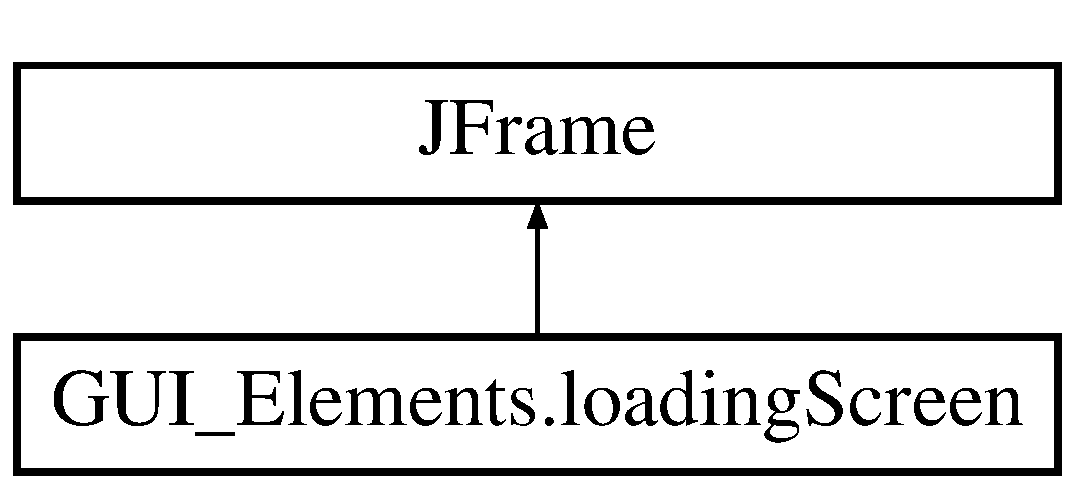
\includegraphics[height=2.000000cm]{class_g_u_i___elements_1_1loading_screen}
\end{center}
\end{figure}
\subsection*{Public Member Functions}
\begin{DoxyCompactItemize}
\item 
\hyperlink{class_g_u_i___elements_1_1loading_screen_a0fc0f5ae4d7ebb422ca36364ccc848b9}{loading\+Screen} (J\+Frame frame, int \+\_\+p)
\item 
void \hyperlink{class_g_u_i___elements_1_1loading_screen_afa7caf6e03de405b8b9c0d6619bac201}{prepare\+Gui} ()
\item 
J\+Progress\+Bar \hyperlink{class_g_u_i___elements_1_1loading_screen_a1cd168a3031086c3d15708213dd11a4b}{get\+Bar} ()
\item 
J\+Frame \hyperlink{class_g_u_i___elements_1_1loading_screen_a565b95f52e78c18e62ccb633ebb9fc49}{get\+Loading} ()
\end{DoxyCompactItemize}


\subsection{Detailed Description}
loading screen that pops up while reading xml file. 

Created by skwow on 11/28/2016. saurabh kumar 2015088 prashant 2015072 

\subsection{Constructor \& Destructor Documentation}
\hypertarget{class_g_u_i___elements_1_1loading_screen_a0fc0f5ae4d7ebb422ca36364ccc848b9}{}\label{class_g_u_i___elements_1_1loading_screen_a0fc0f5ae4d7ebb422ca36364ccc848b9} 
\index{G\+U\+I\+\_\+\+Elements\+::loading\+Screen@{G\+U\+I\+\_\+\+Elements\+::loading\+Screen}!loading\+Screen@{loading\+Screen}}
\index{loading\+Screen@{loading\+Screen}!G\+U\+I\+\_\+\+Elements\+::loading\+Screen@{G\+U\+I\+\_\+\+Elements\+::loading\+Screen}}
\subsubsection{\texorpdfstring{loading\+Screen()}{loadingScreen()}}
{\footnotesize\ttfamily G\+U\+I\+\_\+\+Elements.\+loading\+Screen.\+loading\+Screen (\begin{DoxyParamCaption}\item[{J\+Frame}]{frame,  }\item[{int}]{\+\_\+p }\end{DoxyParamCaption})}

constructor makes gui by taking Jframe, dynamically Example of decorator pattern. 

\subsection{Member Function Documentation}
\hypertarget{class_g_u_i___elements_1_1loading_screen_a1cd168a3031086c3d15708213dd11a4b}{}\label{class_g_u_i___elements_1_1loading_screen_a1cd168a3031086c3d15708213dd11a4b} 
\index{G\+U\+I\+\_\+\+Elements\+::loading\+Screen@{G\+U\+I\+\_\+\+Elements\+::loading\+Screen}!get\+Bar@{get\+Bar}}
\index{get\+Bar@{get\+Bar}!G\+U\+I\+\_\+\+Elements\+::loading\+Screen@{G\+U\+I\+\_\+\+Elements\+::loading\+Screen}}
\subsubsection{\texorpdfstring{get\+Bar()}{getBar()}}
{\footnotesize\ttfamily J\+Progress\+Bar G\+U\+I\+\_\+\+Elements.\+loading\+Screen.\+get\+Bar (\begin{DoxyParamCaption}{ }\end{DoxyParamCaption})}

\hypertarget{class_g_u_i___elements_1_1loading_screen_a565b95f52e78c18e62ccb633ebb9fc49}{}\label{class_g_u_i___elements_1_1loading_screen_a565b95f52e78c18e62ccb633ebb9fc49} 
\index{G\+U\+I\+\_\+\+Elements\+::loading\+Screen@{G\+U\+I\+\_\+\+Elements\+::loading\+Screen}!get\+Loading@{get\+Loading}}
\index{get\+Loading@{get\+Loading}!G\+U\+I\+\_\+\+Elements\+::loading\+Screen@{G\+U\+I\+\_\+\+Elements\+::loading\+Screen}}
\subsubsection{\texorpdfstring{get\+Loading()}{getLoading()}}
{\footnotesize\ttfamily J\+Frame G\+U\+I\+\_\+\+Elements.\+loading\+Screen.\+get\+Loading (\begin{DoxyParamCaption}{ }\end{DoxyParamCaption})}

\hypertarget{class_g_u_i___elements_1_1loading_screen_afa7caf6e03de405b8b9c0d6619bac201}{}\label{class_g_u_i___elements_1_1loading_screen_afa7caf6e03de405b8b9c0d6619bac201} 
\index{G\+U\+I\+\_\+\+Elements\+::loading\+Screen@{G\+U\+I\+\_\+\+Elements\+::loading\+Screen}!prepare\+Gui@{prepare\+Gui}}
\index{prepare\+Gui@{prepare\+Gui}!G\+U\+I\+\_\+\+Elements\+::loading\+Screen@{G\+U\+I\+\_\+\+Elements\+::loading\+Screen}}
\subsubsection{\texorpdfstring{prepare\+Gui()}{prepareGui()}}
{\footnotesize\ttfamily void G\+U\+I\+\_\+\+Elements.\+loading\+Screen.\+prepare\+Gui (\begin{DoxyParamCaption}{ }\end{DoxyParamCaption})}



The documentation for this class was generated from the following file\+:\begin{DoxyCompactItemize}
\item 
C\+:/\+Users/skwow/\+Documents/\+Git\+Hub/\+A\+P\+\_\+\+Project/src/\+G\+U\+I\+\_\+\+Elements/\hyperlink{loading_screen_8java}{loading\+Screen.\+java}\end{DoxyCompactItemize}

\hypertarget{classmain___class_1_1main_class}{}\section{main\+\_\+\+Class.\+main\+Class Class Reference}
\label{classmain___class_1_1main_class}\index{main\+\_\+\+Class.\+main\+Class@{main\+\_\+\+Class.\+main\+Class}}


this is simply the main class  


\subsection*{Static Public Member Functions}
\begin{DoxyCompactItemize}
\item 
static void \hyperlink{classmain___class_1_1main_class_ab3827b8cc7f9a5b8f432ee476700b844}{main} (String\mbox{[}$\,$\mbox{]} args)
\end{DoxyCompactItemize}


\subsection{Detailed Description}
this is simply the main class 

saurabh kumar 2015088 prashant 2015072 

\subsection{Member Function Documentation}
\hypertarget{classmain___class_1_1main_class_ab3827b8cc7f9a5b8f432ee476700b844}{}\label{classmain___class_1_1main_class_ab3827b8cc7f9a5b8f432ee476700b844} 
\index{main\+\_\+\+Class\+::main\+Class@{main\+\_\+\+Class\+::main\+Class}!main@{main}}
\index{main@{main}!main\+\_\+\+Class\+::main\+Class@{main\+\_\+\+Class\+::main\+Class}}
\subsubsection{\texorpdfstring{main()}{main()}}
{\footnotesize\ttfamily static void main\+\_\+\+Class.\+main\+Class.\+main (\begin{DoxyParamCaption}\item[{String \mbox{[}$\,$\mbox{]}}]{args }\end{DoxyParamCaption})\hspace{0.3cm}{\ttfamily [static]}}



The documentation for this class was generated from the following file\+:\begin{DoxyCompactItemize}
\item 
C\+:/\+Users/skwow/\+Documents/\+Git\+Hub/\+A\+P\+\_\+\+Project/src/main\+\_\+\+Class/\hyperlink{main_class_8java}{main\+Class.\+java}\end{DoxyCompactItemize}

\hypertarget{class_g_u_i___elements_1_1my_frame}{}\section{G\+U\+I\+\_\+\+Elements.\+my\+Frame Class Reference}
\label{class_g_u_i___elements_1_1my_frame}\index{G\+U\+I\+\_\+\+Elements.\+my\+Frame@{G\+U\+I\+\_\+\+Elements.\+my\+Frame}}


main G\+UI frame  


Inheritance diagram for G\+U\+I\+\_\+\+Elements.\+my\+Frame\+:\begin{figure}[H]
\begin{center}
\leavevmode
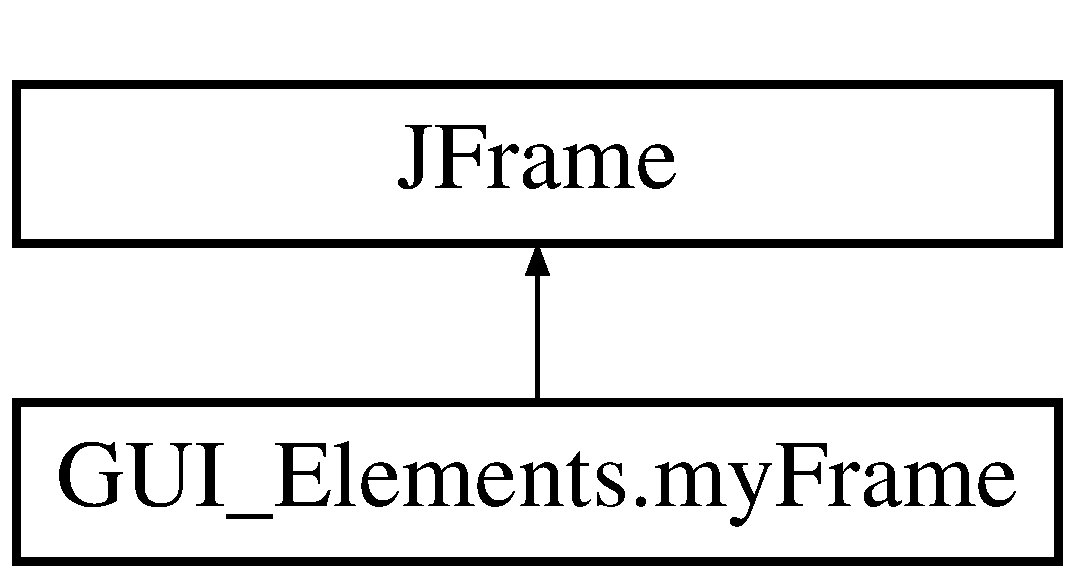
\includegraphics[height=2.000000cm]{class_g_u_i___elements_1_1my_frame}
\end{center}
\end{figure}
\subsection*{Public Member Functions}
\begin{DoxyCompactItemize}
\item 
\hyperlink{class_g_u_i___elements_1_1my_frame_aa440e02a2f616477910624372b55f2fb}{my\+Frame} (\hyperlink{class_g_u_i___elements_1_1my_panel}{my\+Panel} panel)
\item 
void \hyperlink{class_g_u_i___elements_1_1my_frame_a5f5da5b4e114c7aff38f3b4b361bf483}{add\+Draggable} ()
\begin{DoxyCompactList}\small\item\em one can drag it by clicking anywhere on the frame \end{DoxyCompactList}\end{DoxyCompactItemize}


\subsection{Detailed Description}
main G\+UI frame 

Created by skwow on 10/23/2016. 

\subsection{Constructor \& Destructor Documentation}
\hypertarget{class_g_u_i___elements_1_1my_frame_aa440e02a2f616477910624372b55f2fb}{}\label{class_g_u_i___elements_1_1my_frame_aa440e02a2f616477910624372b55f2fb} 
\index{G\+U\+I\+\_\+\+Elements\+::my\+Frame@{G\+U\+I\+\_\+\+Elements\+::my\+Frame}!my\+Frame@{my\+Frame}}
\index{my\+Frame@{my\+Frame}!G\+U\+I\+\_\+\+Elements\+::my\+Frame@{G\+U\+I\+\_\+\+Elements\+::my\+Frame}}
\subsubsection{\texorpdfstring{my\+Frame()}{myFrame()}}
{\footnotesize\ttfamily G\+U\+I\+\_\+\+Elements.\+my\+Frame.\+my\+Frame (\begin{DoxyParamCaption}\item[{\hyperlink{class_g_u_i___elements_1_1my_panel}{my\+Panel}}]{panel }\end{DoxyParamCaption})}



\subsection{Member Function Documentation}
\hypertarget{class_g_u_i___elements_1_1my_frame_a5f5da5b4e114c7aff38f3b4b361bf483}{}\label{class_g_u_i___elements_1_1my_frame_a5f5da5b4e114c7aff38f3b4b361bf483} 
\index{G\+U\+I\+\_\+\+Elements\+::my\+Frame@{G\+U\+I\+\_\+\+Elements\+::my\+Frame}!add\+Draggable@{add\+Draggable}}
\index{add\+Draggable@{add\+Draggable}!G\+U\+I\+\_\+\+Elements\+::my\+Frame@{G\+U\+I\+\_\+\+Elements\+::my\+Frame}}
\subsubsection{\texorpdfstring{add\+Draggable()}{addDraggable()}}
{\footnotesize\ttfamily void G\+U\+I\+\_\+\+Elements.\+my\+Frame.\+add\+Draggable (\begin{DoxyParamCaption}{ }\end{DoxyParamCaption})}



one can drag it by clicking anywhere on the frame 



The documentation for this class was generated from the following file\+:\begin{DoxyCompactItemize}
\item 
C\+:/\+Users/skwow/\+Documents/\+Git\+Hub/\+A\+P\+\_\+\+Project/src/\+G\+U\+I\+\_\+\+Elements/\hyperlink{my_frame_8java}{my\+Frame.\+java}\end{DoxyCompactItemize}

\hypertarget{classutilities_1_1my_own_exeption}{}\section{utilities.\+my\+Own\+Exeption Class Reference}
\label{classutilities_1_1my_own_exeption}\index{utilities.\+my\+Own\+Exeption@{utilities.\+my\+Own\+Exeption}}


this is meant for exception handling by creating dialog box.  


Inheritance diagram for utilities.\+my\+Own\+Exeption\+:\begin{figure}[H]
\begin{center}
\leavevmode
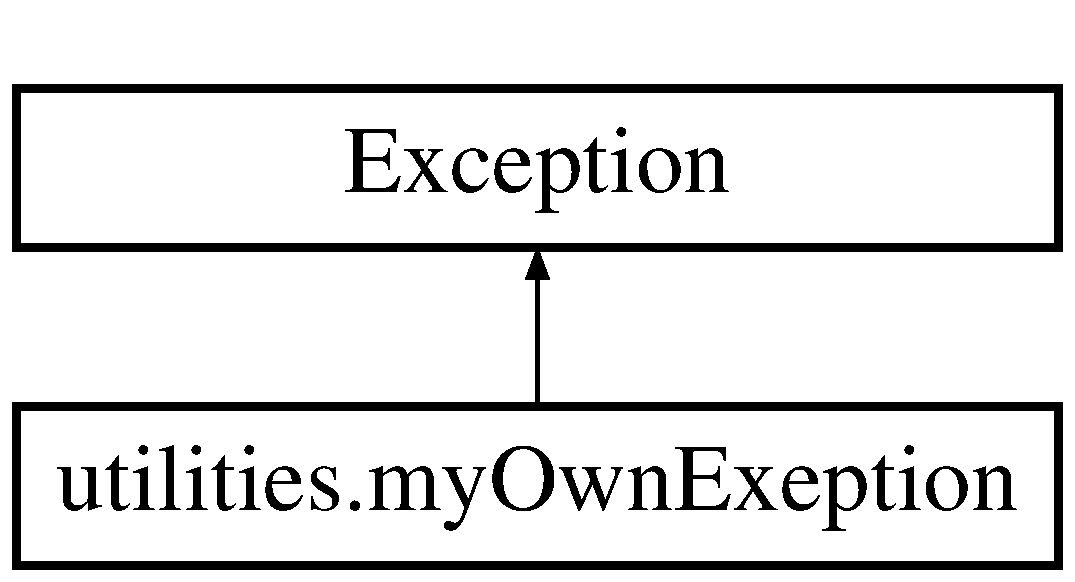
\includegraphics[height=2.000000cm]{classutilities_1_1my_own_exeption}
\end{center}
\end{figure}
\subsection*{Public Member Functions}
\begin{DoxyCompactItemize}
\item 
\hyperlink{classutilities_1_1my_own_exeption_a06cbd6448612ea5d4067e4b2a47acd09}{my\+Own\+Exeption} (String s)
\begin{DoxyCompactList}\small\item\em constructors takes a string \end{DoxyCompactList}\end{DoxyCompactItemize}


\subsection{Detailed Description}
this is meant for exception handling by creating dialog box. 

Created by skwow on 11/21/2016. saurabh kumar 2015088 prashant 2015072 

\subsection{Constructor \& Destructor Documentation}
\hypertarget{classutilities_1_1my_own_exeption_a06cbd6448612ea5d4067e4b2a47acd09}{}\label{classutilities_1_1my_own_exeption_a06cbd6448612ea5d4067e4b2a47acd09} 
\index{utilities\+::my\+Own\+Exeption@{utilities\+::my\+Own\+Exeption}!my\+Own\+Exeption@{my\+Own\+Exeption}}
\index{my\+Own\+Exeption@{my\+Own\+Exeption}!utilities\+::my\+Own\+Exeption@{utilities\+::my\+Own\+Exeption}}
\subsubsection{\texorpdfstring{my\+Own\+Exeption()}{myOwnExeption()}}
{\footnotesize\ttfamily utilities.\+my\+Own\+Exeption.\+my\+Own\+Exeption (\begin{DoxyParamCaption}\item[{String}]{s }\end{DoxyParamCaption})}



constructors takes a string 



The documentation for this class was generated from the following file\+:\begin{DoxyCompactItemize}
\item 
C\+:/\+Users/skwow/\+Documents/\+Git\+Hub/\+A\+P\+\_\+\+Project/src/utilities/\hyperlink{my_own_exeption_8java}{my\+Own\+Exeption.\+java}\end{DoxyCompactItemize}

\hypertarget{class_g_u_i___elements_1_1my_panel}{}\section{G\+U\+I\+\_\+\+Elements.\+my\+Panel Class Reference}
\label{class_g_u_i___elements_1_1my_panel}\index{G\+U\+I\+\_\+\+Elements.\+my\+Panel@{G\+U\+I\+\_\+\+Elements.\+my\+Panel}}


main panel inside \hyperlink{class_g_u_i___elements_1_1my_frame}{my\+Frame}  


\subsection*{Public Member Functions}
\begin{DoxyCompactItemize}
\item 
void \hyperlink{class_g_u_i___elements_1_1my_panel_a0e7ebb816b28db3b3ee0af444afc7b32}{U\+I\+Element\+Factory} ()
\begin{DoxyCompactList}\small\item\em factory pattern for all the gui panel needed by this panel \end{DoxyCompactList}\item 
\hyperlink{class_g_u_i___elements_1_1my_panel_a86c5274d56125927194bdb681d40a3bc}{my\+Panel} ()
\item 
void \hyperlink{class_g_u_i___elements_1_1my_panel_a35817f482730797326227422f83ff9c8}{working\+Of\+Query\+Combo} ()
\begin{DoxyCompactList}\small\item\em switching of panel by selecting type of query \end{DoxyCompactList}\item 
void \hyperlink{class_g_u_i___elements_1_1my_panel_af937a1f734205a826ab7280987c2c420}{working\+Of\+Reset\+Button} ()
\item 
void \hyperlink{class_g_u_i___elements_1_1my_panel_a96d27ef92b9ddceade03b7094e0aefba}{working\+Of\+Search\+Button} ()
\item 
J\+Panel \hyperlink{class_g_u_i___elements_1_1my_panel_abea57f39e7c7b1c89db73d173d71d978}{get\+Panel} ()
\end{DoxyCompactItemize}


\subsection{Detailed Description}
main panel inside \hyperlink{class_g_u_i___elements_1_1my_frame}{my\+Frame} 

Created by skwow on 10/21/2016. 

\subsection{Constructor \& Destructor Documentation}
\hypertarget{class_g_u_i___elements_1_1my_panel_a86c5274d56125927194bdb681d40a3bc}{}\label{class_g_u_i___elements_1_1my_panel_a86c5274d56125927194bdb681d40a3bc} 
\index{G\+U\+I\+\_\+\+Elements\+::my\+Panel@{G\+U\+I\+\_\+\+Elements\+::my\+Panel}!my\+Panel@{my\+Panel}}
\index{my\+Panel@{my\+Panel}!G\+U\+I\+\_\+\+Elements\+::my\+Panel@{G\+U\+I\+\_\+\+Elements\+::my\+Panel}}
\subsubsection{\texorpdfstring{my\+Panel()}{myPanel()}}
{\footnotesize\ttfamily G\+U\+I\+\_\+\+Elements.\+my\+Panel.\+my\+Panel (\begin{DoxyParamCaption}{ }\end{DoxyParamCaption})}



\subsection{Member Function Documentation}
\hypertarget{class_g_u_i___elements_1_1my_panel_abea57f39e7c7b1c89db73d173d71d978}{}\label{class_g_u_i___elements_1_1my_panel_abea57f39e7c7b1c89db73d173d71d978} 
\index{G\+U\+I\+\_\+\+Elements\+::my\+Panel@{G\+U\+I\+\_\+\+Elements\+::my\+Panel}!get\+Panel@{get\+Panel}}
\index{get\+Panel@{get\+Panel}!G\+U\+I\+\_\+\+Elements\+::my\+Panel@{G\+U\+I\+\_\+\+Elements\+::my\+Panel}}
\subsubsection{\texorpdfstring{get\+Panel()}{getPanel()}}
{\footnotesize\ttfamily J\+Panel G\+U\+I\+\_\+\+Elements.\+my\+Panel.\+get\+Panel (\begin{DoxyParamCaption}{ }\end{DoxyParamCaption})}

\hypertarget{class_g_u_i___elements_1_1my_panel_a0e7ebb816b28db3b3ee0af444afc7b32}{}\label{class_g_u_i___elements_1_1my_panel_a0e7ebb816b28db3b3ee0af444afc7b32} 
\index{G\+U\+I\+\_\+\+Elements\+::my\+Panel@{G\+U\+I\+\_\+\+Elements\+::my\+Panel}!U\+I\+Element\+Factory@{U\+I\+Element\+Factory}}
\index{U\+I\+Element\+Factory@{U\+I\+Element\+Factory}!G\+U\+I\+\_\+\+Elements\+::my\+Panel@{G\+U\+I\+\_\+\+Elements\+::my\+Panel}}
\subsubsection{\texorpdfstring{U\+I\+Element\+Factory()}{UIElementFactory()}}
{\footnotesize\ttfamily void G\+U\+I\+\_\+\+Elements.\+my\+Panel.\+U\+I\+Element\+Factory (\begin{DoxyParamCaption}{ }\end{DoxyParamCaption})}



factory pattern for all the gui panel needed by this panel 

\hypertarget{class_g_u_i___elements_1_1my_panel_a35817f482730797326227422f83ff9c8}{}\label{class_g_u_i___elements_1_1my_panel_a35817f482730797326227422f83ff9c8} 
\index{G\+U\+I\+\_\+\+Elements\+::my\+Panel@{G\+U\+I\+\_\+\+Elements\+::my\+Panel}!working\+Of\+Query\+Combo@{working\+Of\+Query\+Combo}}
\index{working\+Of\+Query\+Combo@{working\+Of\+Query\+Combo}!G\+U\+I\+\_\+\+Elements\+::my\+Panel@{G\+U\+I\+\_\+\+Elements\+::my\+Panel}}
\subsubsection{\texorpdfstring{working\+Of\+Query\+Combo()}{workingOfQueryCombo()}}
{\footnotesize\ttfamily void G\+U\+I\+\_\+\+Elements.\+my\+Panel.\+working\+Of\+Query\+Combo (\begin{DoxyParamCaption}{ }\end{DoxyParamCaption})}



switching of panel by selecting type of query 

\hypertarget{class_g_u_i___elements_1_1my_panel_af937a1f734205a826ab7280987c2c420}{}\label{class_g_u_i___elements_1_1my_panel_af937a1f734205a826ab7280987c2c420} 
\index{G\+U\+I\+\_\+\+Elements\+::my\+Panel@{G\+U\+I\+\_\+\+Elements\+::my\+Panel}!working\+Of\+Reset\+Button@{working\+Of\+Reset\+Button}}
\index{working\+Of\+Reset\+Button@{working\+Of\+Reset\+Button}!G\+U\+I\+\_\+\+Elements\+::my\+Panel@{G\+U\+I\+\_\+\+Elements\+::my\+Panel}}
\subsubsection{\texorpdfstring{working\+Of\+Reset\+Button()}{workingOfResetButton()}}
{\footnotesize\ttfamily void G\+U\+I\+\_\+\+Elements.\+my\+Panel.\+working\+Of\+Reset\+Button (\begin{DoxyParamCaption}{ }\end{DoxyParamCaption})}

\hypertarget{class_g_u_i___elements_1_1my_panel_a96d27ef92b9ddceade03b7094e0aefba}{}\label{class_g_u_i___elements_1_1my_panel_a96d27ef92b9ddceade03b7094e0aefba} 
\index{G\+U\+I\+\_\+\+Elements\+::my\+Panel@{G\+U\+I\+\_\+\+Elements\+::my\+Panel}!working\+Of\+Search\+Button@{working\+Of\+Search\+Button}}
\index{working\+Of\+Search\+Button@{working\+Of\+Search\+Button}!G\+U\+I\+\_\+\+Elements\+::my\+Panel@{G\+U\+I\+\_\+\+Elements\+::my\+Panel}}
\subsubsection{\texorpdfstring{working\+Of\+Search\+Button()}{workingOfSearchButton()}}
{\footnotesize\ttfamily void G\+U\+I\+\_\+\+Elements.\+my\+Panel.\+working\+Of\+Search\+Button (\begin{DoxyParamCaption}{ }\end{DoxyParamCaption})}



The documentation for this class was generated from the following file\+:\begin{DoxyCompactItemize}
\item 
C\+:/\+Users/skwow/\+Documents/\+Git\+Hub/\+A\+P\+\_\+\+Project/src/\+G\+U\+I\+\_\+\+Elements/\hyperlink{my_panel_8java}{my\+Panel.\+java}\end{DoxyCompactItemize}

\hypertarget{class_g_u_i___elements_1_1my_query1_panel}{}\section{G\+U\+I\+\_\+\+Elements.\+my\+Query1\+Panel Class Reference}
\label{class_g_u_i___elements_1_1my_query1_panel}\index{G\+U\+I\+\_\+\+Elements.\+my\+Query1\+Panel@{G\+U\+I\+\_\+\+Elements.\+my\+Query1\+Panel}}
Inheritance diagram for G\+U\+I\+\_\+\+Elements.\+my\+Query1\+Panel\+:\begin{figure}[H]
\begin{center}
\leavevmode
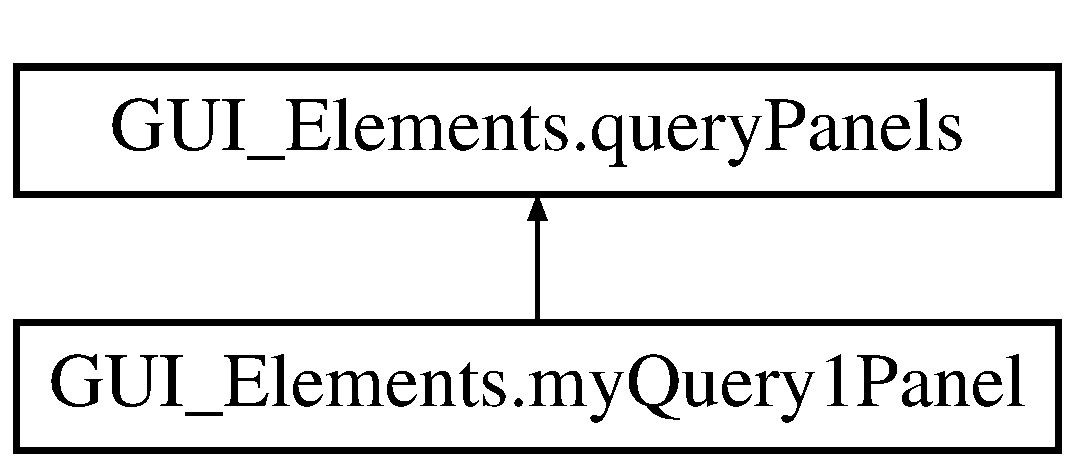
\includegraphics[height=2.000000cm]{class_g_u_i___elements_1_1my_query1_panel}
\end{center}
\end{figure}
\subsection*{Public Member Functions}
\begin{DoxyCompactItemize}
\item 
\hyperlink{class_g_u_i___elements_1_1my_query1_panel_a327650227b1692cbbc2f8ef90a133afc}{my\+Query1\+Panel} ()
\begin{DoxyCompactList}\small\item\em constructor initiates the skeleton of interface \end{DoxyCompactList}\item 
void \hyperlink{class_g_u_i___elements_1_1my_query1_panel_ae73a3545beb076fc0f7114e6175bd423}{colorize} ()
\item 
void \hyperlink{class_g_u_i___elements_1_1my_query1_panel_a0b16368de01ed227e625524541a455ea}{prepare\+Buttons} ()
\end{DoxyCompactItemize}
\subsection*{Protected Attributes}
\begin{DoxyCompactItemize}
\item 
J\+Panel \hyperlink{class_g_u_i___elements_1_1my_query1_panel_ab923a9c569a07cdb10332b944e871903}{panel2} =new J\+Panel(new Grid\+Bag\+Layout())
\item 
J\+Button \hyperlink{class_g_u_i___elements_1_1my_query1_panel_a258a18ffc0a0a2614b3029be4765a067}{reset\+Button}
\item 
J\+Text\+Field \hyperlink{class_g_u_i___elements_1_1my_query1_panel_a960fb72a45e85925b931852ce4b218eb}{since\+Year\+Teaxt\+Field}
\item 
J\+Combo\+Box \hyperlink{class_g_u_i___elements_1_1my_query1_panel_a8327a7218462c60f0b0b9eeed6ba392c}{year\+Combo}
\item 
Checkbox \hyperlink{class_g_u_i___elements_1_1my_query1_panel_a021a96e74cad421c5dda3f8b98e3feb6}{chk\+Sort\+By\+Year}
\item 
Checkbox\+Group \hyperlink{class_g_u_i___elements_1_1my_query1_panel_a349792b04363355dc174bfbad3ac6422}{sort}
\end{DoxyCompactItemize}


\subsection{Detailed Description}
Created by skwow on 10/23/2016. saurabh kumar 2015088 prashant 2015072 

\subsection{Constructor \& Destructor Documentation}
\hypertarget{class_g_u_i___elements_1_1my_query1_panel_a327650227b1692cbbc2f8ef90a133afc}{}\label{class_g_u_i___elements_1_1my_query1_panel_a327650227b1692cbbc2f8ef90a133afc} 
\index{G\+U\+I\+\_\+\+Elements\+::my\+Query1\+Panel@{G\+U\+I\+\_\+\+Elements\+::my\+Query1\+Panel}!my\+Query1\+Panel@{my\+Query1\+Panel}}
\index{my\+Query1\+Panel@{my\+Query1\+Panel}!G\+U\+I\+\_\+\+Elements\+::my\+Query1\+Panel@{G\+U\+I\+\_\+\+Elements\+::my\+Query1\+Panel}}
\subsubsection{\texorpdfstring{my\+Query1\+Panel()}{myQuery1Panel()}}
{\footnotesize\ttfamily G\+U\+I\+\_\+\+Elements.\+my\+Query1\+Panel.\+my\+Query1\+Panel (\begin{DoxyParamCaption}{ }\end{DoxyParamCaption})}



constructor initiates the skeleton of interface 



\subsection{Member Function Documentation}
\hypertarget{class_g_u_i___elements_1_1my_query1_panel_ae73a3545beb076fc0f7114e6175bd423}{}\label{class_g_u_i___elements_1_1my_query1_panel_ae73a3545beb076fc0f7114e6175bd423} 
\index{G\+U\+I\+\_\+\+Elements\+::my\+Query1\+Panel@{G\+U\+I\+\_\+\+Elements\+::my\+Query1\+Panel}!colorize@{colorize}}
\index{colorize@{colorize}!G\+U\+I\+\_\+\+Elements\+::my\+Query1\+Panel@{G\+U\+I\+\_\+\+Elements\+::my\+Query1\+Panel}}
\subsubsection{\texorpdfstring{colorize()}{colorize()}}
{\footnotesize\ttfamily void G\+U\+I\+\_\+\+Elements.\+my\+Query1\+Panel.\+colorize (\begin{DoxyParamCaption}{ }\end{DoxyParamCaption})}

\hypertarget{class_g_u_i___elements_1_1my_query1_panel_a0b16368de01ed227e625524541a455ea}{}\label{class_g_u_i___elements_1_1my_query1_panel_a0b16368de01ed227e625524541a455ea} 
\index{G\+U\+I\+\_\+\+Elements\+::my\+Query1\+Panel@{G\+U\+I\+\_\+\+Elements\+::my\+Query1\+Panel}!prepare\+Buttons@{prepare\+Buttons}}
\index{prepare\+Buttons@{prepare\+Buttons}!G\+U\+I\+\_\+\+Elements\+::my\+Query1\+Panel@{G\+U\+I\+\_\+\+Elements\+::my\+Query1\+Panel}}
\subsubsection{\texorpdfstring{prepare\+Buttons()}{prepareButtons()}}
{\footnotesize\ttfamily void G\+U\+I\+\_\+\+Elements.\+my\+Query1\+Panel.\+prepare\+Buttons (\begin{DoxyParamCaption}{ }\end{DoxyParamCaption})}



\subsection{Member Data Documentation}
\hypertarget{class_g_u_i___elements_1_1my_query1_panel_a021a96e74cad421c5dda3f8b98e3feb6}{}\label{class_g_u_i___elements_1_1my_query1_panel_a021a96e74cad421c5dda3f8b98e3feb6} 
\index{G\+U\+I\+\_\+\+Elements\+::my\+Query1\+Panel@{G\+U\+I\+\_\+\+Elements\+::my\+Query1\+Panel}!chk\+Sort\+By\+Year@{chk\+Sort\+By\+Year}}
\index{chk\+Sort\+By\+Year@{chk\+Sort\+By\+Year}!G\+U\+I\+\_\+\+Elements\+::my\+Query1\+Panel@{G\+U\+I\+\_\+\+Elements\+::my\+Query1\+Panel}}
\subsubsection{\texorpdfstring{chk\+Sort\+By\+Year}{chkSortByYear}}
{\footnotesize\ttfamily Checkbox G\+U\+I\+\_\+\+Elements.\+my\+Query1\+Panel.\+chk\+Sort\+By\+Year\hspace{0.3cm}{\ttfamily [protected]}}

\hypertarget{class_g_u_i___elements_1_1my_query1_panel_ab923a9c569a07cdb10332b944e871903}{}\label{class_g_u_i___elements_1_1my_query1_panel_ab923a9c569a07cdb10332b944e871903} 
\index{G\+U\+I\+\_\+\+Elements\+::my\+Query1\+Panel@{G\+U\+I\+\_\+\+Elements\+::my\+Query1\+Panel}!panel2@{panel2}}
\index{panel2@{panel2}!G\+U\+I\+\_\+\+Elements\+::my\+Query1\+Panel@{G\+U\+I\+\_\+\+Elements\+::my\+Query1\+Panel}}
\subsubsection{\texorpdfstring{panel2}{panel2}}
{\footnotesize\ttfamily J\+Panel G\+U\+I\+\_\+\+Elements.\+my\+Query1\+Panel.\+panel2 =new J\+Panel(new Grid\+Bag\+Layout())\hspace{0.3cm}{\ttfamily [protected]}}

\hypertarget{class_g_u_i___elements_1_1my_query1_panel_a258a18ffc0a0a2614b3029be4765a067}{}\label{class_g_u_i___elements_1_1my_query1_panel_a258a18ffc0a0a2614b3029be4765a067} 
\index{G\+U\+I\+\_\+\+Elements\+::my\+Query1\+Panel@{G\+U\+I\+\_\+\+Elements\+::my\+Query1\+Panel}!reset\+Button@{reset\+Button}}
\index{reset\+Button@{reset\+Button}!G\+U\+I\+\_\+\+Elements\+::my\+Query1\+Panel@{G\+U\+I\+\_\+\+Elements\+::my\+Query1\+Panel}}
\subsubsection{\texorpdfstring{reset\+Button}{resetButton}}
{\footnotesize\ttfamily J\+Button G\+U\+I\+\_\+\+Elements.\+my\+Query1\+Panel.\+reset\+Button\hspace{0.3cm}{\ttfamily [protected]}}

\hypertarget{class_g_u_i___elements_1_1my_query1_panel_a960fb72a45e85925b931852ce4b218eb}{}\label{class_g_u_i___elements_1_1my_query1_panel_a960fb72a45e85925b931852ce4b218eb} 
\index{G\+U\+I\+\_\+\+Elements\+::my\+Query1\+Panel@{G\+U\+I\+\_\+\+Elements\+::my\+Query1\+Panel}!since\+Year\+Teaxt\+Field@{since\+Year\+Teaxt\+Field}}
\index{since\+Year\+Teaxt\+Field@{since\+Year\+Teaxt\+Field}!G\+U\+I\+\_\+\+Elements\+::my\+Query1\+Panel@{G\+U\+I\+\_\+\+Elements\+::my\+Query1\+Panel}}
\subsubsection{\texorpdfstring{since\+Year\+Teaxt\+Field}{sinceYearTeaxtField}}
{\footnotesize\ttfamily J\+Text\+Field G\+U\+I\+\_\+\+Elements.\+my\+Query1\+Panel.\+since\+Year\+Teaxt\+Field\hspace{0.3cm}{\ttfamily [protected]}}

\hypertarget{class_g_u_i___elements_1_1my_query1_panel_a349792b04363355dc174bfbad3ac6422}{}\label{class_g_u_i___elements_1_1my_query1_panel_a349792b04363355dc174bfbad3ac6422} 
\index{G\+U\+I\+\_\+\+Elements\+::my\+Query1\+Panel@{G\+U\+I\+\_\+\+Elements\+::my\+Query1\+Panel}!sort@{sort}}
\index{sort@{sort}!G\+U\+I\+\_\+\+Elements\+::my\+Query1\+Panel@{G\+U\+I\+\_\+\+Elements\+::my\+Query1\+Panel}}
\subsubsection{\texorpdfstring{sort}{sort}}
{\footnotesize\ttfamily Checkbox\+Group G\+U\+I\+\_\+\+Elements.\+my\+Query1\+Panel.\+sort\hspace{0.3cm}{\ttfamily [protected]}}

\hypertarget{class_g_u_i___elements_1_1my_query1_panel_a8327a7218462c60f0b0b9eeed6ba392c}{}\label{class_g_u_i___elements_1_1my_query1_panel_a8327a7218462c60f0b0b9eeed6ba392c} 
\index{G\+U\+I\+\_\+\+Elements\+::my\+Query1\+Panel@{G\+U\+I\+\_\+\+Elements\+::my\+Query1\+Panel}!year\+Combo@{year\+Combo}}
\index{year\+Combo@{year\+Combo}!G\+U\+I\+\_\+\+Elements\+::my\+Query1\+Panel@{G\+U\+I\+\_\+\+Elements\+::my\+Query1\+Panel}}
\subsubsection{\texorpdfstring{year\+Combo}{yearCombo}}
{\footnotesize\ttfamily J\+Combo\+Box G\+U\+I\+\_\+\+Elements.\+my\+Query1\+Panel.\+year\+Combo\hspace{0.3cm}{\ttfamily [protected]}}



The documentation for this class was generated from the following file\+:\begin{DoxyCompactItemize}
\item 
C\+:/\+Users/skwow/\+Documents/\+Git\+Hub/\+A\+P\+\_\+\+Project/src/\+G\+U\+I\+\_\+\+Elements/\hyperlink{my_query1_panel_8java}{my\+Query1\+Panel.\+java}\end{DoxyCompactItemize}

\hypertarget{class_g_u_i___elements_1_1my_query2_panel}{}\section{G\+U\+I\+\_\+\+Elements.\+my\+Query2\+Panel Class Reference}
\label{class_g_u_i___elements_1_1my_query2_panel}\index{G\+U\+I\+\_\+\+Elements.\+my\+Query2\+Panel@{G\+U\+I\+\_\+\+Elements.\+my\+Query2\+Panel}}
Inheritance diagram for G\+U\+I\+\_\+\+Elements.\+my\+Query2\+Panel\+:\begin{figure}[H]
\begin{center}
\leavevmode
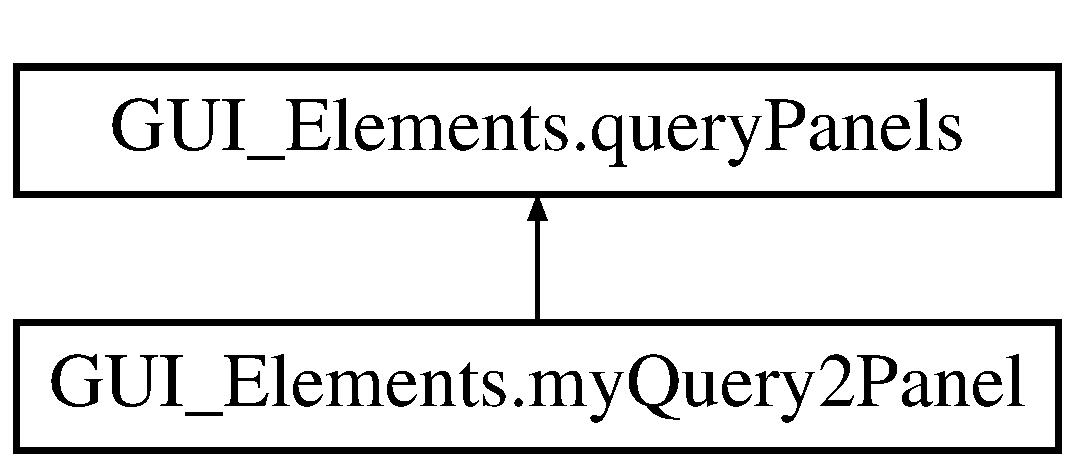
\includegraphics[height=2.000000cm]{class_g_u_i___elements_1_1my_query2_panel}
\end{center}
\end{figure}
\subsection*{Public Member Functions}
\begin{DoxyCompactItemize}
\item 
\hyperlink{class_g_u_i___elements_1_1my_query2_panel_ac3fc56f3c07e6c0bc190e6e5f4b3a73b}{my\+Query2\+Panel} ()
\begin{DoxyCompactList}\small\item\em constructor initiates the skeleton of interface \end{DoxyCompactList}\item 
void \hyperlink{class_g_u_i___elements_1_1my_query2_panel_a047854ba4d510a94711c82daa2ca81bb}{colorize} ()
\item 
void \hyperlink{class_g_u_i___elements_1_1my_query2_panel_ad99535b063e2d3ff044560245837eecf}{prepare\+Gui} ()
\item 
void \hyperlink{class_g_u_i___elements_1_1my_query2_panel_a71b3714eb5b1a303b8229ef240415524}{prepare\+Buttons} ()
\item 
void \hyperlink{class_g_u_i___elements_1_1my_query2_panel_afed162247688600c698720b4ed2351c7}{working\+Of\+Buttons} ()
\item 
J\+Panel \hyperlink{class_g_u_i___elements_1_1my_query2_panel_a45bac12608ab0c76e4583fad0aa17cb0}{get\+Panel} ()
\end{DoxyCompactItemize}


\subsection{Detailed Description}
Created by skwow on 10/27/2016. 

\subsection{Constructor \& Destructor Documentation}
\hypertarget{class_g_u_i___elements_1_1my_query2_panel_ac3fc56f3c07e6c0bc190e6e5f4b3a73b}{}\label{class_g_u_i___elements_1_1my_query2_panel_ac3fc56f3c07e6c0bc190e6e5f4b3a73b} 
\index{G\+U\+I\+\_\+\+Elements\+::my\+Query2\+Panel@{G\+U\+I\+\_\+\+Elements\+::my\+Query2\+Panel}!my\+Query2\+Panel@{my\+Query2\+Panel}}
\index{my\+Query2\+Panel@{my\+Query2\+Panel}!G\+U\+I\+\_\+\+Elements\+::my\+Query2\+Panel@{G\+U\+I\+\_\+\+Elements\+::my\+Query2\+Panel}}
\subsubsection{\texorpdfstring{my\+Query2\+Panel()}{myQuery2Panel()}}
{\footnotesize\ttfamily G\+U\+I\+\_\+\+Elements.\+my\+Query2\+Panel.\+my\+Query2\+Panel (\begin{DoxyParamCaption}{ }\end{DoxyParamCaption})}



constructor initiates the skeleton of interface 



\subsection{Member Function Documentation}
\hypertarget{class_g_u_i___elements_1_1my_query2_panel_a047854ba4d510a94711c82daa2ca81bb}{}\label{class_g_u_i___elements_1_1my_query2_panel_a047854ba4d510a94711c82daa2ca81bb} 
\index{G\+U\+I\+\_\+\+Elements\+::my\+Query2\+Panel@{G\+U\+I\+\_\+\+Elements\+::my\+Query2\+Panel}!colorize@{colorize}}
\index{colorize@{colorize}!G\+U\+I\+\_\+\+Elements\+::my\+Query2\+Panel@{G\+U\+I\+\_\+\+Elements\+::my\+Query2\+Panel}}
\subsubsection{\texorpdfstring{colorize()}{colorize()}}
{\footnotesize\ttfamily void G\+U\+I\+\_\+\+Elements.\+my\+Query2\+Panel.\+colorize (\begin{DoxyParamCaption}{ }\end{DoxyParamCaption})}

\hypertarget{class_g_u_i___elements_1_1my_query2_panel_a45bac12608ab0c76e4583fad0aa17cb0}{}\label{class_g_u_i___elements_1_1my_query2_panel_a45bac12608ab0c76e4583fad0aa17cb0} 
\index{G\+U\+I\+\_\+\+Elements\+::my\+Query2\+Panel@{G\+U\+I\+\_\+\+Elements\+::my\+Query2\+Panel}!get\+Panel@{get\+Panel}}
\index{get\+Panel@{get\+Panel}!G\+U\+I\+\_\+\+Elements\+::my\+Query2\+Panel@{G\+U\+I\+\_\+\+Elements\+::my\+Query2\+Panel}}
\subsubsection{\texorpdfstring{get\+Panel()}{getPanel()}}
{\footnotesize\ttfamily J\+Panel G\+U\+I\+\_\+\+Elements.\+my\+Query2\+Panel.\+get\+Panel (\begin{DoxyParamCaption}{ }\end{DoxyParamCaption})}

\hypertarget{class_g_u_i___elements_1_1my_query2_panel_a71b3714eb5b1a303b8229ef240415524}{}\label{class_g_u_i___elements_1_1my_query2_panel_a71b3714eb5b1a303b8229ef240415524} 
\index{G\+U\+I\+\_\+\+Elements\+::my\+Query2\+Panel@{G\+U\+I\+\_\+\+Elements\+::my\+Query2\+Panel}!prepare\+Buttons@{prepare\+Buttons}}
\index{prepare\+Buttons@{prepare\+Buttons}!G\+U\+I\+\_\+\+Elements\+::my\+Query2\+Panel@{G\+U\+I\+\_\+\+Elements\+::my\+Query2\+Panel}}
\subsubsection{\texorpdfstring{prepare\+Buttons()}{prepareButtons()}}
{\footnotesize\ttfamily void G\+U\+I\+\_\+\+Elements.\+my\+Query2\+Panel.\+prepare\+Buttons (\begin{DoxyParamCaption}{ }\end{DoxyParamCaption})}

\hypertarget{class_g_u_i___elements_1_1my_query2_panel_ad99535b063e2d3ff044560245837eecf}{}\label{class_g_u_i___elements_1_1my_query2_panel_ad99535b063e2d3ff044560245837eecf} 
\index{G\+U\+I\+\_\+\+Elements\+::my\+Query2\+Panel@{G\+U\+I\+\_\+\+Elements\+::my\+Query2\+Panel}!prepare\+Gui@{prepare\+Gui}}
\index{prepare\+Gui@{prepare\+Gui}!G\+U\+I\+\_\+\+Elements\+::my\+Query2\+Panel@{G\+U\+I\+\_\+\+Elements\+::my\+Query2\+Panel}}
\subsubsection{\texorpdfstring{prepare\+Gui()}{prepareGui()}}
{\footnotesize\ttfamily void G\+U\+I\+\_\+\+Elements.\+my\+Query2\+Panel.\+prepare\+Gui (\begin{DoxyParamCaption}{ }\end{DoxyParamCaption})}

\hypertarget{class_g_u_i___elements_1_1my_query2_panel_afed162247688600c698720b4ed2351c7}{}\label{class_g_u_i___elements_1_1my_query2_panel_afed162247688600c698720b4ed2351c7} 
\index{G\+U\+I\+\_\+\+Elements\+::my\+Query2\+Panel@{G\+U\+I\+\_\+\+Elements\+::my\+Query2\+Panel}!working\+Of\+Buttons@{working\+Of\+Buttons}}
\index{working\+Of\+Buttons@{working\+Of\+Buttons}!G\+U\+I\+\_\+\+Elements\+::my\+Query2\+Panel@{G\+U\+I\+\_\+\+Elements\+::my\+Query2\+Panel}}
\subsubsection{\texorpdfstring{working\+Of\+Buttons()}{workingOfButtons()}}
{\footnotesize\ttfamily void G\+U\+I\+\_\+\+Elements.\+my\+Query2\+Panel.\+working\+Of\+Buttons (\begin{DoxyParamCaption}{ }\end{DoxyParamCaption})}



The documentation for this class was generated from the following file\+:\begin{DoxyCompactItemize}
\item 
C\+:/\+Users/skwow/\+Documents/\+Git\+Hub/\+A\+P\+\_\+\+Project/src/\+G\+U\+I\+\_\+\+Elements/\hyperlink{my_query2_panel_8java}{my\+Query2\+Panel.\+java}\end{DoxyCompactItemize}

\hypertarget{class_g_u_i___elements_1_1my_query3_panel}{}\section{G\+U\+I\+\_\+\+Elements.\+my\+Query3\+Panel Class Reference}
\label{class_g_u_i___elements_1_1my_query3_panel}\index{G\+U\+I\+\_\+\+Elements.\+my\+Query3\+Panel@{G\+U\+I\+\_\+\+Elements.\+my\+Query3\+Panel}}
Inheritance diagram for G\+U\+I\+\_\+\+Elements.\+my\+Query3\+Panel\+:\begin{figure}[H]
\begin{center}
\leavevmode
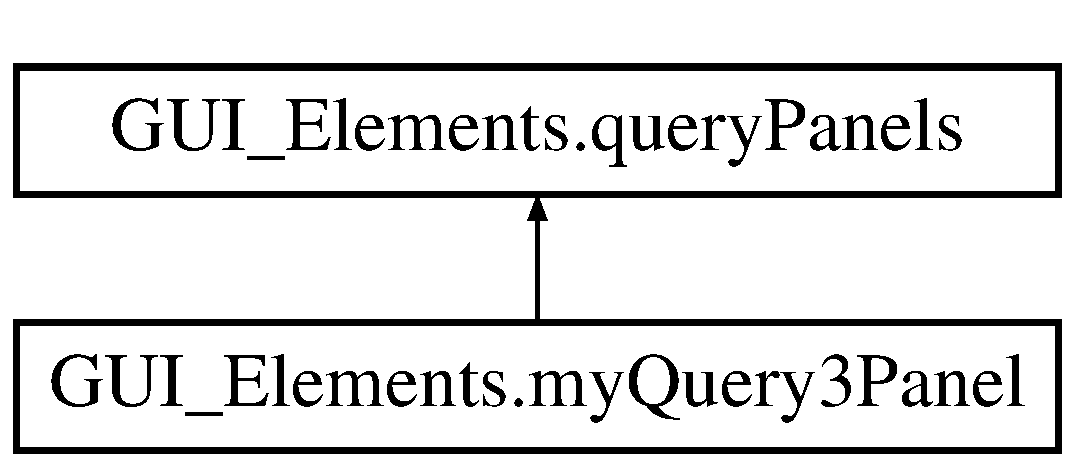
\includegraphics[height=2.000000cm]{class_g_u_i___elements_1_1my_query3_panel}
\end{center}
\end{figure}
\subsection*{Public Member Functions}
\begin{DoxyCompactItemize}
\item 
\hyperlink{class_g_u_i___elements_1_1my_query3_panel_a6d672bacf210e53a00e148a27a4ea2b8}{my\+Query3\+Panel} ()
\begin{DoxyCompactList}\small\item\em constructor initiates the skeleton of interface \end{DoxyCompactList}\item 
void \hyperlink{class_g_u_i___elements_1_1my_query3_panel_ad3c37661350b9ed95d749ca33450ff69}{colorize} ()
\item 
void \hyperlink{class_g_u_i___elements_1_1my_query3_panel_a0edd26c1cd0bd4b5621508c32b89d362}{prepare\+Gui} ()
\item 
void \hyperlink{class_g_u_i___elements_1_1my_query3_panel_a51ae30aafd90618c99d3b6b67734ddd3}{prepare\+Buttons} ()
\item 
void \hyperlink{class_g_u_i___elements_1_1my_query3_panel_a09bd68ef59c9ffadd8e72abf72186533}{working\+Of\+Buttons} ()
\item 
J\+Panel \hyperlink{class_g_u_i___elements_1_1my_query3_panel_ad792ef80368c829d32e9329a2ba7bb17}{get\+Panel} ()
\end{DoxyCompactItemize}


\subsection{Detailed Description}
Created by skwow on 10/27/2016. saurabh kumar 2015088 prashant 2015072 

\subsection{Constructor \& Destructor Documentation}
\hypertarget{class_g_u_i___elements_1_1my_query3_panel_a6d672bacf210e53a00e148a27a4ea2b8}{}\label{class_g_u_i___elements_1_1my_query3_panel_a6d672bacf210e53a00e148a27a4ea2b8} 
\index{G\+U\+I\+\_\+\+Elements\+::my\+Query3\+Panel@{G\+U\+I\+\_\+\+Elements\+::my\+Query3\+Panel}!my\+Query3\+Panel@{my\+Query3\+Panel}}
\index{my\+Query3\+Panel@{my\+Query3\+Panel}!G\+U\+I\+\_\+\+Elements\+::my\+Query3\+Panel@{G\+U\+I\+\_\+\+Elements\+::my\+Query3\+Panel}}
\subsubsection{\texorpdfstring{my\+Query3\+Panel()}{myQuery3Panel()}}
{\footnotesize\ttfamily G\+U\+I\+\_\+\+Elements.\+my\+Query3\+Panel.\+my\+Query3\+Panel (\begin{DoxyParamCaption}{ }\end{DoxyParamCaption})}



constructor initiates the skeleton of interface 



\subsection{Member Function Documentation}
\hypertarget{class_g_u_i___elements_1_1my_query3_panel_ad3c37661350b9ed95d749ca33450ff69}{}\label{class_g_u_i___elements_1_1my_query3_panel_ad3c37661350b9ed95d749ca33450ff69} 
\index{G\+U\+I\+\_\+\+Elements\+::my\+Query3\+Panel@{G\+U\+I\+\_\+\+Elements\+::my\+Query3\+Panel}!colorize@{colorize}}
\index{colorize@{colorize}!G\+U\+I\+\_\+\+Elements\+::my\+Query3\+Panel@{G\+U\+I\+\_\+\+Elements\+::my\+Query3\+Panel}}
\subsubsection{\texorpdfstring{colorize()}{colorize()}}
{\footnotesize\ttfamily void G\+U\+I\+\_\+\+Elements.\+my\+Query3\+Panel.\+colorize (\begin{DoxyParamCaption}{ }\end{DoxyParamCaption})}

\hypertarget{class_g_u_i___elements_1_1my_query3_panel_ad792ef80368c829d32e9329a2ba7bb17}{}\label{class_g_u_i___elements_1_1my_query3_panel_ad792ef80368c829d32e9329a2ba7bb17} 
\index{G\+U\+I\+\_\+\+Elements\+::my\+Query3\+Panel@{G\+U\+I\+\_\+\+Elements\+::my\+Query3\+Panel}!get\+Panel@{get\+Panel}}
\index{get\+Panel@{get\+Panel}!G\+U\+I\+\_\+\+Elements\+::my\+Query3\+Panel@{G\+U\+I\+\_\+\+Elements\+::my\+Query3\+Panel}}
\subsubsection{\texorpdfstring{get\+Panel()}{getPanel()}}
{\footnotesize\ttfamily J\+Panel G\+U\+I\+\_\+\+Elements.\+my\+Query3\+Panel.\+get\+Panel (\begin{DoxyParamCaption}{ }\end{DoxyParamCaption})}

\hypertarget{class_g_u_i___elements_1_1my_query3_panel_a51ae30aafd90618c99d3b6b67734ddd3}{}\label{class_g_u_i___elements_1_1my_query3_panel_a51ae30aafd90618c99d3b6b67734ddd3} 
\index{G\+U\+I\+\_\+\+Elements\+::my\+Query3\+Panel@{G\+U\+I\+\_\+\+Elements\+::my\+Query3\+Panel}!prepare\+Buttons@{prepare\+Buttons}}
\index{prepare\+Buttons@{prepare\+Buttons}!G\+U\+I\+\_\+\+Elements\+::my\+Query3\+Panel@{G\+U\+I\+\_\+\+Elements\+::my\+Query3\+Panel}}
\subsubsection{\texorpdfstring{prepare\+Buttons()}{prepareButtons()}}
{\footnotesize\ttfamily void G\+U\+I\+\_\+\+Elements.\+my\+Query3\+Panel.\+prepare\+Buttons (\begin{DoxyParamCaption}{ }\end{DoxyParamCaption})}

\hypertarget{class_g_u_i___elements_1_1my_query3_panel_a0edd26c1cd0bd4b5621508c32b89d362}{}\label{class_g_u_i___elements_1_1my_query3_panel_a0edd26c1cd0bd4b5621508c32b89d362} 
\index{G\+U\+I\+\_\+\+Elements\+::my\+Query3\+Panel@{G\+U\+I\+\_\+\+Elements\+::my\+Query3\+Panel}!prepare\+Gui@{prepare\+Gui}}
\index{prepare\+Gui@{prepare\+Gui}!G\+U\+I\+\_\+\+Elements\+::my\+Query3\+Panel@{G\+U\+I\+\_\+\+Elements\+::my\+Query3\+Panel}}
\subsubsection{\texorpdfstring{prepare\+Gui()}{prepareGui()}}
{\footnotesize\ttfamily void G\+U\+I\+\_\+\+Elements.\+my\+Query3\+Panel.\+prepare\+Gui (\begin{DoxyParamCaption}{ }\end{DoxyParamCaption})}

\hypertarget{class_g_u_i___elements_1_1my_query3_panel_a09bd68ef59c9ffadd8e72abf72186533}{}\label{class_g_u_i___elements_1_1my_query3_panel_a09bd68ef59c9ffadd8e72abf72186533} 
\index{G\+U\+I\+\_\+\+Elements\+::my\+Query3\+Panel@{G\+U\+I\+\_\+\+Elements\+::my\+Query3\+Panel}!working\+Of\+Buttons@{working\+Of\+Buttons}}
\index{working\+Of\+Buttons@{working\+Of\+Buttons}!G\+U\+I\+\_\+\+Elements\+::my\+Query3\+Panel@{G\+U\+I\+\_\+\+Elements\+::my\+Query3\+Panel}}
\subsubsection{\texorpdfstring{working\+Of\+Buttons()}{workingOfButtons()}}
{\footnotesize\ttfamily void G\+U\+I\+\_\+\+Elements.\+my\+Query3\+Panel.\+working\+Of\+Buttons (\begin{DoxyParamCaption}{ }\end{DoxyParamCaption})}



The documentation for this class was generated from the following file\+:\begin{DoxyCompactItemize}
\item 
C\+:/\+Users/skwow/\+Documents/\+Git\+Hub/\+A\+P\+\_\+\+Project/src/\+G\+U\+I\+\_\+\+Elements/\hyperlink{my_query3_panel_8java}{my\+Query3\+Panel.\+java}\end{DoxyCompactItemize}

\hypertarget{classutilities_1_1parser}{}\section{utilities.\+parser Class Reference}
\label{classutilities_1_1parser}\index{utilities.\+parser@{utilities.\+parser}}


this class perses the xml class  


Inheritance diagram for utilities.\+parser\+:\begin{figure}[H]
\begin{center}
\leavevmode
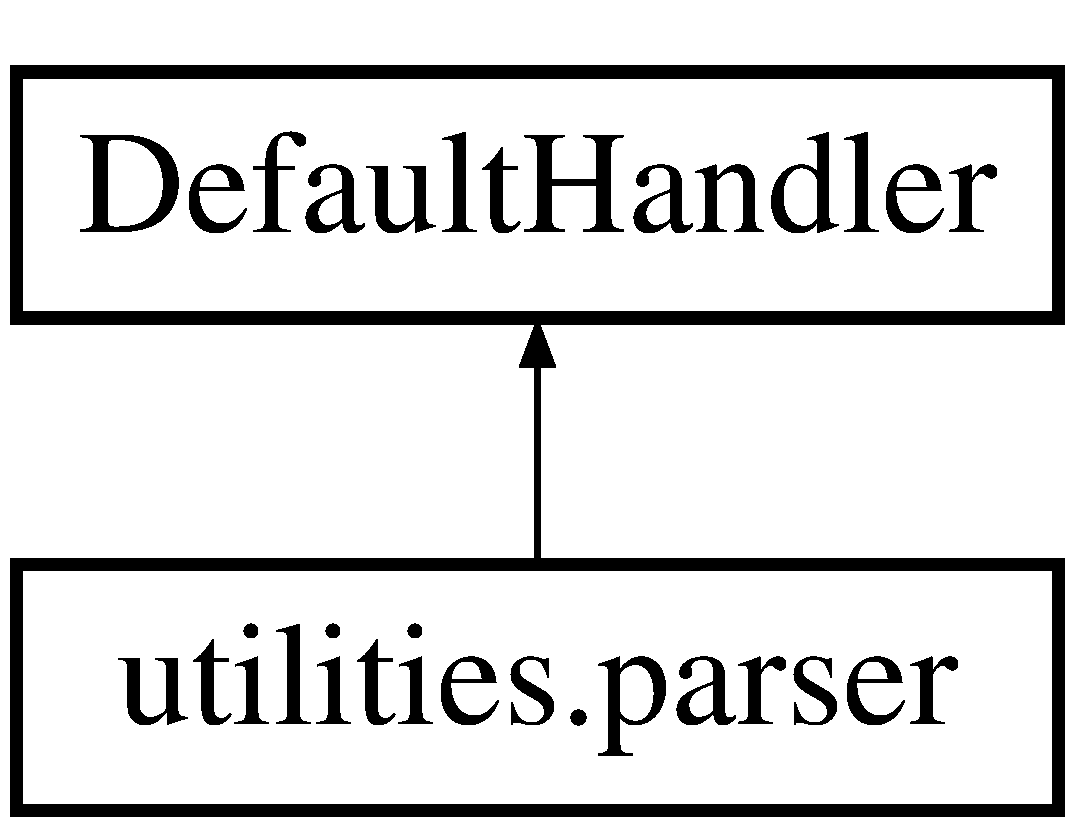
\includegraphics[height=2.000000cm]{classutilities_1_1parser}
\end{center}
\end{figure}
\subsection*{Public Member Functions}
\begin{DoxyCompactItemize}
\item 
void \hyperlink{classutilities_1_1parser_ae11f73c41940e9ee2d05b95ab2fb9435}{parse} ()
\item 
void \hyperlink{classutilities_1_1parser_a89378ec321afe4275ae9a6f5833e5fb9}{start\+Element} (String uri, String local\+Name, String q\+Name, Attributes attributes)  throws S\+A\+X\+Exception 
\item 
void \hyperlink{classutilities_1_1parser_a63a7843809987e45e5bb9bb790a1c8ff}{end\+Element} (String uri, String local\+Name, String q\+Name)  throws S\+A\+X\+Exception 
\item 
void \hyperlink{classutilities_1_1parser_aaf564dc89d2e86903538e014323d1482}{characters} (char ch\mbox{[}$\,$\mbox{]}, int start, int length)  throws S\+A\+X\+Exception 
\end{DoxyCompactItemize}
\subsection*{Static Public Member Functions}
\begin{DoxyCompactItemize}
\item 
static \hyperlink{classutilities_1_1parser}{parser} \hyperlink{classutilities_1_1parser_aca9b03d52069091a9fbe48ca5723a52c}{get\+Instance} ()
\end{DoxyCompactItemize}


\subsection{Detailed Description}
this class perses the xml class 

Created by skwow on 11/8/2016. 

\subsection{Member Function Documentation}
\hypertarget{classutilities_1_1parser_aaf564dc89d2e86903538e014323d1482}{}\label{classutilities_1_1parser_aaf564dc89d2e86903538e014323d1482} 
\index{utilities\+::parser@{utilities\+::parser}!characters@{characters}}
\index{characters@{characters}!utilities\+::parser@{utilities\+::parser}}
\subsubsection{\texorpdfstring{characters()}{characters()}}
{\footnotesize\ttfamily void utilities.\+parser.\+characters (\begin{DoxyParamCaption}\item[{char}]{ch\mbox{[}$\,$\mbox{]},  }\item[{int}]{start,  }\item[{int}]{length }\end{DoxyParamCaption}) throws S\+A\+X\+Exception}

\hypertarget{classutilities_1_1parser_a63a7843809987e45e5bb9bb790a1c8ff}{}\label{classutilities_1_1parser_a63a7843809987e45e5bb9bb790a1c8ff} 
\index{utilities\+::parser@{utilities\+::parser}!end\+Element@{end\+Element}}
\index{end\+Element@{end\+Element}!utilities\+::parser@{utilities\+::parser}}
\subsubsection{\texorpdfstring{end\+Element()}{endElement()}}
{\footnotesize\ttfamily void utilities.\+parser.\+end\+Element (\begin{DoxyParamCaption}\item[{String}]{uri,  }\item[{String}]{local\+Name,  }\item[{String}]{q\+Name }\end{DoxyParamCaption}) throws S\+A\+X\+Exception}

\hypertarget{classutilities_1_1parser_aca9b03d52069091a9fbe48ca5723a52c}{}\label{classutilities_1_1parser_aca9b03d52069091a9fbe48ca5723a52c} 
\index{utilities\+::parser@{utilities\+::parser}!get\+Instance@{get\+Instance}}
\index{get\+Instance@{get\+Instance}!utilities\+::parser@{utilities\+::parser}}
\subsubsection{\texorpdfstring{get\+Instance()}{getInstance()}}
{\footnotesize\ttfamily static \hyperlink{classutilities_1_1parser}{parser} utilities.\+parser.\+get\+Instance (\begin{DoxyParamCaption}{ }\end{DoxyParamCaption})\hspace{0.3cm}{\ttfamily [static]}}

\hypertarget{classutilities_1_1parser_ae11f73c41940e9ee2d05b95ab2fb9435}{}\label{classutilities_1_1parser_ae11f73c41940e9ee2d05b95ab2fb9435} 
\index{utilities\+::parser@{utilities\+::parser}!parse@{parse}}
\index{parse@{parse}!utilities\+::parser@{utilities\+::parser}}
\subsubsection{\texorpdfstring{parse()}{parse()}}
{\footnotesize\ttfamily void utilities.\+parser.\+parse (\begin{DoxyParamCaption}{ }\end{DoxyParamCaption})}

\hypertarget{classutilities_1_1parser_a89378ec321afe4275ae9a6f5833e5fb9}{}\label{classutilities_1_1parser_a89378ec321afe4275ae9a6f5833e5fb9} 
\index{utilities\+::parser@{utilities\+::parser}!start\+Element@{start\+Element}}
\index{start\+Element@{start\+Element}!utilities\+::parser@{utilities\+::parser}}
\subsubsection{\texorpdfstring{start\+Element()}{startElement()}}
{\footnotesize\ttfamily void utilities.\+parser.\+start\+Element (\begin{DoxyParamCaption}\item[{String}]{uri,  }\item[{String}]{local\+Name,  }\item[{String}]{q\+Name,  }\item[{Attributes}]{attributes }\end{DoxyParamCaption}) throws S\+A\+X\+Exception}



The documentation for this class was generated from the following file\+:\begin{DoxyCompactItemize}
\item 
C\+:/\+Users/skwow/\+Documents/\+Git\+Hub/\+A\+P\+\_\+\+Project/src/utilities/\hyperlink{parser_8java}{parser.\+java}\end{DoxyCompactItemize}

\hypertarget{class_data_1_1publishables}{}\section{Data.\+publishables Class Reference}
\label{class_data_1_1publishables}\index{Data.\+publishables@{Data.\+publishables}}


publishale comprises of all thethigs in the xml  


Inheritance diagram for Data.\+publishables\+:\begin{figure}[H]
\begin{center}
\leavevmode
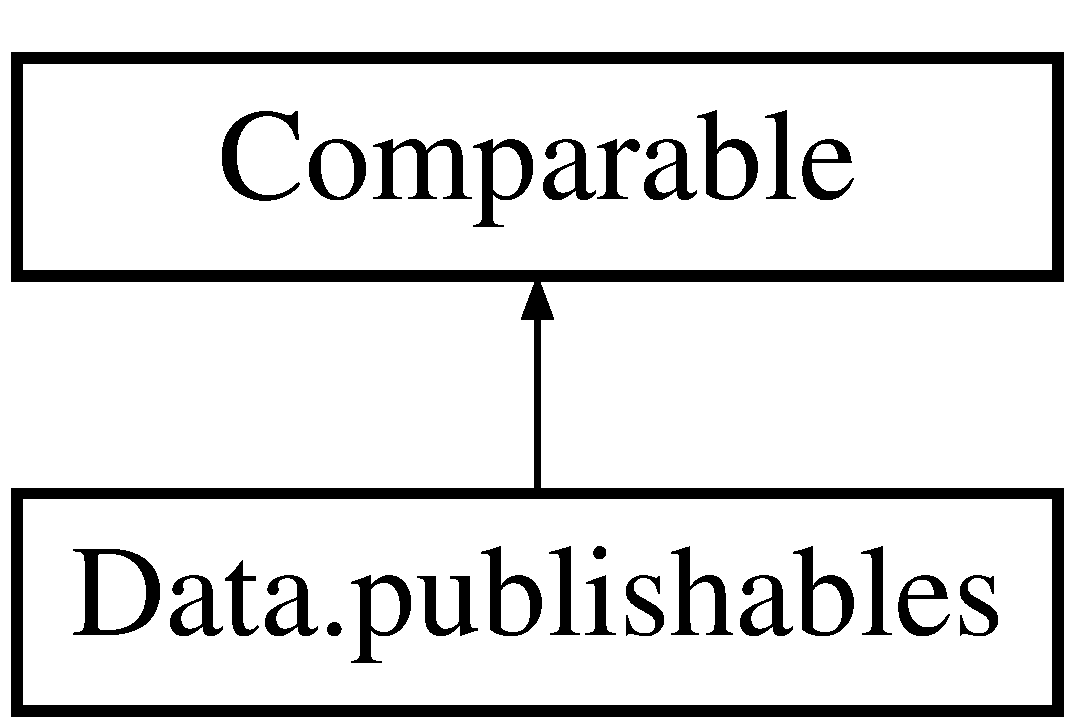
\includegraphics[height=2.000000cm]{class_data_1_1publishables}
\end{center}
\end{figure}
\subsection*{Public Member Functions}
\begin{DoxyCompactItemize}
\item 
\hyperlink{class_data_1_1publishables_aceabba690b9f11b724b7ca0bb1bd6ed9}{publishables} ()
\item 
void \hyperlink{class_data_1_1publishables_a3d53c9a74e1dad13a2f12b7c4e521956}{set\+Title} (String title)
\item 
void \hyperlink{class_data_1_1publishables_aa1ccf268dc89410fa9ab554470c66817}{set\+Year} (int year)
\item 
void \hyperlink{class_data_1_1publishables_ad75ef8fda848ce0c92bd3a0cffbb7cd5}{set\+Volume} (String volume)
\item 
void \hyperlink{class_data_1_1publishables_a5f50216c1c3ec50ec46fb866ee3aa584}{set\+Pages} (String pages)
\item 
void \hyperlink{class_data_1_1publishables_a735b41a8df635fd719eae7927ed81329}{set\+Journal\+\_\+booktitle} (String journal\+\_\+booktitle)
\item 
void \hyperlink{class_data_1_1publishables_afefb90428e6d1ce4f699b4a4a10da4fa}{add\+Author} (String \+\_\+author)
\item 
void \hyperlink{class_data_1_1publishables_a1ab3287a7eada2b725f7e1d735d235fa}{add\+Url} (String \+\_\+url)
\item 
String \hyperlink{class_data_1_1publishables_adb157b10f5a2a4fb9a842cc85e32f54b}{get\+Author} ()
\item 
String \hyperlink{class_data_1_1publishables_a8e829e500e2f0aa65e57c344cc1afb7c}{get\+Url} ()
\item 
String \hyperlink{class_data_1_1publishables_a8b14020ff568a02776ffe674eac0fcba}{get\+Title} ()
\item 
int \hyperlink{class_data_1_1publishables_a75f9f918753d279ce0eb81e4956931df}{get\+Year} ()
\item 
String \hyperlink{class_data_1_1publishables_a6b3f36e7f557b5d3fc7c44d6975318a2}{get\+Volume} ()
\item 
String \hyperlink{class_data_1_1publishables_af657673a106cc994008f104f62f639ba}{get\+Pages} ()
\item 
String \hyperlink{class_data_1_1publishables_a7a83ab5278085e3fb9ea8f5b57860b0d}{get\+Journal\+\_\+booktitle} ()
\item 
Array\+List$<$ String $>$ \hyperlink{class_data_1_1publishables_a309ee4a6e0475636adf30390f9edfb10}{get\+Raw\+Author} ()
\item 
int \hyperlink{class_data_1_1publishables_a05a1e076d45e561c6e3d3f745849f650}{compare\+To} (Object o)
\begin{DoxyCompactList}\small\item\em compares on the basis of year \end{DoxyCompactList}\item 
String \hyperlink{class_data_1_1publishables_a61c53fb0b33bffd164b4cbba2b5add43}{to\+String} ()
\end{DoxyCompactItemize}


\subsection{Detailed Description}
publishale comprises of all thethigs in the xml 

Created by skwow on 10/14/2016. saurabh kumar 2015088 prashant 2015072 

\subsection{Constructor \& Destructor Documentation}
\hypertarget{class_data_1_1publishables_aceabba690b9f11b724b7ca0bb1bd6ed9}{}\label{class_data_1_1publishables_aceabba690b9f11b724b7ca0bb1bd6ed9} 
\index{Data\+::publishables@{Data\+::publishables}!publishables@{publishables}}
\index{publishables@{publishables}!Data\+::publishables@{Data\+::publishables}}
\subsubsection{\texorpdfstring{publishables()}{publishables()}}
{\footnotesize\ttfamily Data.\+publishables.\+publishables (\begin{DoxyParamCaption}{ }\end{DoxyParamCaption})}



\subsection{Member Function Documentation}
\hypertarget{class_data_1_1publishables_afefb90428e6d1ce4f699b4a4a10da4fa}{}\label{class_data_1_1publishables_afefb90428e6d1ce4f699b4a4a10da4fa} 
\index{Data\+::publishables@{Data\+::publishables}!add\+Author@{add\+Author}}
\index{add\+Author@{add\+Author}!Data\+::publishables@{Data\+::publishables}}
\subsubsection{\texorpdfstring{add\+Author()}{addAuthor()}}
{\footnotesize\ttfamily void Data.\+publishables.\+add\+Author (\begin{DoxyParamCaption}\item[{String}]{\+\_\+author }\end{DoxyParamCaption})}

\hypertarget{class_data_1_1publishables_a1ab3287a7eada2b725f7e1d735d235fa}{}\label{class_data_1_1publishables_a1ab3287a7eada2b725f7e1d735d235fa} 
\index{Data\+::publishables@{Data\+::publishables}!add\+Url@{add\+Url}}
\index{add\+Url@{add\+Url}!Data\+::publishables@{Data\+::publishables}}
\subsubsection{\texorpdfstring{add\+Url()}{addUrl()}}
{\footnotesize\ttfamily void Data.\+publishables.\+add\+Url (\begin{DoxyParamCaption}\item[{String}]{\+\_\+url }\end{DoxyParamCaption})}

\hypertarget{class_data_1_1publishables_a05a1e076d45e561c6e3d3f745849f650}{}\label{class_data_1_1publishables_a05a1e076d45e561c6e3d3f745849f650} 
\index{Data\+::publishables@{Data\+::publishables}!compare\+To@{compare\+To}}
\index{compare\+To@{compare\+To}!Data\+::publishables@{Data\+::publishables}}
\subsubsection{\texorpdfstring{compare\+To()}{compareTo()}}
{\footnotesize\ttfamily int Data.\+publishables.\+compare\+To (\begin{DoxyParamCaption}\item[{Object}]{o }\end{DoxyParamCaption})}



compares on the basis of year 

\hypertarget{class_data_1_1publishables_adb157b10f5a2a4fb9a842cc85e32f54b}{}\label{class_data_1_1publishables_adb157b10f5a2a4fb9a842cc85e32f54b} 
\index{Data\+::publishables@{Data\+::publishables}!get\+Author@{get\+Author}}
\index{get\+Author@{get\+Author}!Data\+::publishables@{Data\+::publishables}}
\subsubsection{\texorpdfstring{get\+Author()}{getAuthor()}}
{\footnotesize\ttfamily String Data.\+publishables.\+get\+Author (\begin{DoxyParamCaption}{ }\end{DoxyParamCaption})}

\hypertarget{class_data_1_1publishables_a7a83ab5278085e3fb9ea8f5b57860b0d}{}\label{class_data_1_1publishables_a7a83ab5278085e3fb9ea8f5b57860b0d} 
\index{Data\+::publishables@{Data\+::publishables}!get\+Journal\+\_\+booktitle@{get\+Journal\+\_\+booktitle}}
\index{get\+Journal\+\_\+booktitle@{get\+Journal\+\_\+booktitle}!Data\+::publishables@{Data\+::publishables}}
\subsubsection{\texorpdfstring{get\+Journal\+\_\+booktitle()}{getJournal\_booktitle()}}
{\footnotesize\ttfamily String Data.\+publishables.\+get\+Journal\+\_\+booktitle (\begin{DoxyParamCaption}{ }\end{DoxyParamCaption})}

\hypertarget{class_data_1_1publishables_af657673a106cc994008f104f62f639ba}{}\label{class_data_1_1publishables_af657673a106cc994008f104f62f639ba} 
\index{Data\+::publishables@{Data\+::publishables}!get\+Pages@{get\+Pages}}
\index{get\+Pages@{get\+Pages}!Data\+::publishables@{Data\+::publishables}}
\subsubsection{\texorpdfstring{get\+Pages()}{getPages()}}
{\footnotesize\ttfamily String Data.\+publishables.\+get\+Pages (\begin{DoxyParamCaption}{ }\end{DoxyParamCaption})}

\hypertarget{class_data_1_1publishables_a309ee4a6e0475636adf30390f9edfb10}{}\label{class_data_1_1publishables_a309ee4a6e0475636adf30390f9edfb10} 
\index{Data\+::publishables@{Data\+::publishables}!get\+Raw\+Author@{get\+Raw\+Author}}
\index{get\+Raw\+Author@{get\+Raw\+Author}!Data\+::publishables@{Data\+::publishables}}
\subsubsection{\texorpdfstring{get\+Raw\+Author()}{getRawAuthor()}}
{\footnotesize\ttfamily Array\+List$<$String$>$ Data.\+publishables.\+get\+Raw\+Author (\begin{DoxyParamCaption}{ }\end{DoxyParamCaption})}

\hypertarget{class_data_1_1publishables_a8b14020ff568a02776ffe674eac0fcba}{}\label{class_data_1_1publishables_a8b14020ff568a02776ffe674eac0fcba} 
\index{Data\+::publishables@{Data\+::publishables}!get\+Title@{get\+Title}}
\index{get\+Title@{get\+Title}!Data\+::publishables@{Data\+::publishables}}
\subsubsection{\texorpdfstring{get\+Title()}{getTitle()}}
{\footnotesize\ttfamily String Data.\+publishables.\+get\+Title (\begin{DoxyParamCaption}{ }\end{DoxyParamCaption})}

\hypertarget{class_data_1_1publishables_a8e829e500e2f0aa65e57c344cc1afb7c}{}\label{class_data_1_1publishables_a8e829e500e2f0aa65e57c344cc1afb7c} 
\index{Data\+::publishables@{Data\+::publishables}!get\+Url@{get\+Url}}
\index{get\+Url@{get\+Url}!Data\+::publishables@{Data\+::publishables}}
\subsubsection{\texorpdfstring{get\+Url()}{getUrl()}}
{\footnotesize\ttfamily String Data.\+publishables.\+get\+Url (\begin{DoxyParamCaption}{ }\end{DoxyParamCaption})}

\hypertarget{class_data_1_1publishables_a6b3f36e7f557b5d3fc7c44d6975318a2}{}\label{class_data_1_1publishables_a6b3f36e7f557b5d3fc7c44d6975318a2} 
\index{Data\+::publishables@{Data\+::publishables}!get\+Volume@{get\+Volume}}
\index{get\+Volume@{get\+Volume}!Data\+::publishables@{Data\+::publishables}}
\subsubsection{\texorpdfstring{get\+Volume()}{getVolume()}}
{\footnotesize\ttfamily String Data.\+publishables.\+get\+Volume (\begin{DoxyParamCaption}{ }\end{DoxyParamCaption})}

\hypertarget{class_data_1_1publishables_a75f9f918753d279ce0eb81e4956931df}{}\label{class_data_1_1publishables_a75f9f918753d279ce0eb81e4956931df} 
\index{Data\+::publishables@{Data\+::publishables}!get\+Year@{get\+Year}}
\index{get\+Year@{get\+Year}!Data\+::publishables@{Data\+::publishables}}
\subsubsection{\texorpdfstring{get\+Year()}{getYear()}}
{\footnotesize\ttfamily int Data.\+publishables.\+get\+Year (\begin{DoxyParamCaption}{ }\end{DoxyParamCaption})}

\hypertarget{class_data_1_1publishables_a735b41a8df635fd719eae7927ed81329}{}\label{class_data_1_1publishables_a735b41a8df635fd719eae7927ed81329} 
\index{Data\+::publishables@{Data\+::publishables}!set\+Journal\+\_\+booktitle@{set\+Journal\+\_\+booktitle}}
\index{set\+Journal\+\_\+booktitle@{set\+Journal\+\_\+booktitle}!Data\+::publishables@{Data\+::publishables}}
\subsubsection{\texorpdfstring{set\+Journal\+\_\+booktitle()}{setJournal\_booktitle()}}
{\footnotesize\ttfamily void Data.\+publishables.\+set\+Journal\+\_\+booktitle (\begin{DoxyParamCaption}\item[{String}]{journal\+\_\+booktitle }\end{DoxyParamCaption})}

\hypertarget{class_data_1_1publishables_a5f50216c1c3ec50ec46fb866ee3aa584}{}\label{class_data_1_1publishables_a5f50216c1c3ec50ec46fb866ee3aa584} 
\index{Data\+::publishables@{Data\+::publishables}!set\+Pages@{set\+Pages}}
\index{set\+Pages@{set\+Pages}!Data\+::publishables@{Data\+::publishables}}
\subsubsection{\texorpdfstring{set\+Pages()}{setPages()}}
{\footnotesize\ttfamily void Data.\+publishables.\+set\+Pages (\begin{DoxyParamCaption}\item[{String}]{pages }\end{DoxyParamCaption})}

\hypertarget{class_data_1_1publishables_a3d53c9a74e1dad13a2f12b7c4e521956}{}\label{class_data_1_1publishables_a3d53c9a74e1dad13a2f12b7c4e521956} 
\index{Data\+::publishables@{Data\+::publishables}!set\+Title@{set\+Title}}
\index{set\+Title@{set\+Title}!Data\+::publishables@{Data\+::publishables}}
\subsubsection{\texorpdfstring{set\+Title()}{setTitle()}}
{\footnotesize\ttfamily void Data.\+publishables.\+set\+Title (\begin{DoxyParamCaption}\item[{String}]{title }\end{DoxyParamCaption})}

\hypertarget{class_data_1_1publishables_ad75ef8fda848ce0c92bd3a0cffbb7cd5}{}\label{class_data_1_1publishables_ad75ef8fda848ce0c92bd3a0cffbb7cd5} 
\index{Data\+::publishables@{Data\+::publishables}!set\+Volume@{set\+Volume}}
\index{set\+Volume@{set\+Volume}!Data\+::publishables@{Data\+::publishables}}
\subsubsection{\texorpdfstring{set\+Volume()}{setVolume()}}
{\footnotesize\ttfamily void Data.\+publishables.\+set\+Volume (\begin{DoxyParamCaption}\item[{String}]{volume }\end{DoxyParamCaption})}

\hypertarget{class_data_1_1publishables_aa1ccf268dc89410fa9ab554470c66817}{}\label{class_data_1_1publishables_aa1ccf268dc89410fa9ab554470c66817} 
\index{Data\+::publishables@{Data\+::publishables}!set\+Year@{set\+Year}}
\index{set\+Year@{set\+Year}!Data\+::publishables@{Data\+::publishables}}
\subsubsection{\texorpdfstring{set\+Year()}{setYear()}}
{\footnotesize\ttfamily void Data.\+publishables.\+set\+Year (\begin{DoxyParamCaption}\item[{int}]{year }\end{DoxyParamCaption})}

\hypertarget{class_data_1_1publishables_a61c53fb0b33bffd164b4cbba2b5add43}{}\label{class_data_1_1publishables_a61c53fb0b33bffd164b4cbba2b5add43} 
\index{Data\+::publishables@{Data\+::publishables}!to\+String@{to\+String}}
\index{to\+String@{to\+String}!Data\+::publishables@{Data\+::publishables}}
\subsubsection{\texorpdfstring{to\+String()}{toString()}}
{\footnotesize\ttfamily String Data.\+publishables.\+to\+String (\begin{DoxyParamCaption}{ }\end{DoxyParamCaption})}



The documentation for this class was generated from the following file\+:\begin{DoxyCompactItemize}
\item 
C\+:/\+Users/skwow/\+Documents/\+Git\+Hub/\+A\+P\+\_\+\+Project/src/\+Data/\hyperlink{publishables_8java}{publishables.\+java}\end{DoxyCompactItemize}

\hypertarget{classquery__handlers_1_1query1_handler}{}\section{query\+\_\+handlers.\+query1\+Handler Class Reference}
\label{classquery__handlers_1_1query1_handler}\index{query\+\_\+handlers.\+query1\+Handler@{query\+\_\+handlers.\+query1\+Handler}}
Inheritance diagram for query\+\_\+handlers.\+query1\+Handler\+:\begin{figure}[H]
\begin{center}
\leavevmode
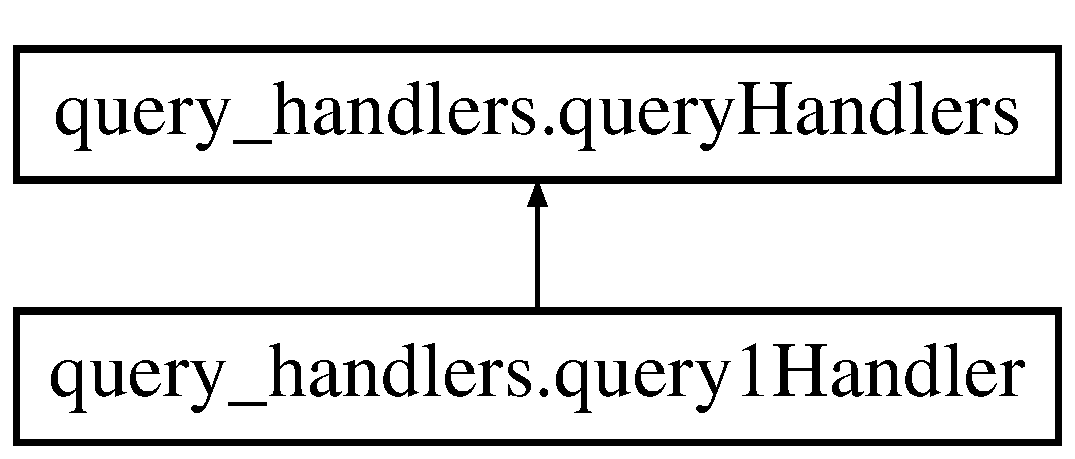
\includegraphics[height=2.000000cm]{classquery__handlers_1_1query1_handler}
\end{center}
\end{figure}
\subsection*{Public Member Functions}
\begin{DoxyCompactItemize}
\item 
\hyperlink{classquery__handlers_1_1query1_handler_a6fe01c044940a164a6c56149fd031131}{query1\+Handler} (String \+\_\+name\+\_\+title, int \+\_\+sortby, int \+\_\+nametitle, int \+\_\+from, int \+\_\+to)
\begin{DoxyCompactList}\small\item\em constructor \end{DoxyCompactList}\item 
void \hyperlink{classquery__handlers_1_1query1_handler_a6e9b752a4ad27626e66dd07bd45661df}{do\+Work} ()
\item 
void \hyperlink{classquery__handlers_1_1query1_handler_ad31be63c673088813821cb1150c8506e}{sort} ()
\item 
void \hyperlink{classquery__handlers_1_1query1_handler_a139b0b15be5b2a7ac0b58a70906fb2a0}{add} (\hyperlink{class_data_1_1publishables}{publishables} x)
\item 
void \hyperlink{classquery__handlers_1_1query1_handler_adb0e49911128d6a1e710cace36a4fae0}{print} ()
\end{DoxyCompactItemize}


\subsection{Detailed Description}
Created by skwow on 10/18/2016. saurabh kumar 2015088 prashant 2015072 

\subsection{Constructor \& Destructor Documentation}
\hypertarget{classquery__handlers_1_1query1_handler_a6fe01c044940a164a6c56149fd031131}{}\label{classquery__handlers_1_1query1_handler_a6fe01c044940a164a6c56149fd031131} 
\index{query\+\_\+handlers\+::query1\+Handler@{query\+\_\+handlers\+::query1\+Handler}!query1\+Handler@{query1\+Handler}}
\index{query1\+Handler@{query1\+Handler}!query\+\_\+handlers\+::query1\+Handler@{query\+\_\+handlers\+::query1\+Handler}}
\subsubsection{\texorpdfstring{query1\+Handler()}{query1Handler()}}
{\footnotesize\ttfamily query\+\_\+handlers.\+query1\+Handler.\+query1\+Handler (\begin{DoxyParamCaption}\item[{String}]{\+\_\+name\+\_\+title,  }\item[{int}]{\+\_\+sortby,  }\item[{int}]{\+\_\+nametitle,  }\item[{int}]{\+\_\+from,  }\item[{int}]{\+\_\+to }\end{DoxyParamCaption})}



constructor 



\subsection{Member Function Documentation}
\hypertarget{classquery__handlers_1_1query1_handler_a139b0b15be5b2a7ac0b58a70906fb2a0}{}\label{classquery__handlers_1_1query1_handler_a139b0b15be5b2a7ac0b58a70906fb2a0} 
\index{query\+\_\+handlers\+::query1\+Handler@{query\+\_\+handlers\+::query1\+Handler}!add@{add}}
\index{add@{add}!query\+\_\+handlers\+::query1\+Handler@{query\+\_\+handlers\+::query1\+Handler}}
\subsubsection{\texorpdfstring{add()}{add()}}
{\footnotesize\ttfamily void query\+\_\+handlers.\+query1\+Handler.\+add (\begin{DoxyParamCaption}\item[{\hyperlink{class_data_1_1publishables}{publishables}}]{x }\end{DoxyParamCaption})}

\hypertarget{classquery__handlers_1_1query1_handler_a6e9b752a4ad27626e66dd07bd45661df}{}\label{classquery__handlers_1_1query1_handler_a6e9b752a4ad27626e66dd07bd45661df} 
\index{query\+\_\+handlers\+::query1\+Handler@{query\+\_\+handlers\+::query1\+Handler}!do\+Work@{do\+Work}}
\index{do\+Work@{do\+Work}!query\+\_\+handlers\+::query1\+Handler@{query\+\_\+handlers\+::query1\+Handler}}
\subsubsection{\texorpdfstring{do\+Work()}{doWork()}}
{\footnotesize\ttfamily void query\+\_\+handlers.\+query1\+Handler.\+do\+Work (\begin{DoxyParamCaption}{ }\end{DoxyParamCaption})}

\hypertarget{classquery__handlers_1_1query1_handler_adb0e49911128d6a1e710cace36a4fae0}{}\label{classquery__handlers_1_1query1_handler_adb0e49911128d6a1e710cace36a4fae0} 
\index{query\+\_\+handlers\+::query1\+Handler@{query\+\_\+handlers\+::query1\+Handler}!print@{print}}
\index{print@{print}!query\+\_\+handlers\+::query1\+Handler@{query\+\_\+handlers\+::query1\+Handler}}
\subsubsection{\texorpdfstring{print()}{print()}}
{\footnotesize\ttfamily void query\+\_\+handlers.\+query1\+Handler.\+print (\begin{DoxyParamCaption}{ }\end{DoxyParamCaption})}

\hypertarget{classquery__handlers_1_1query1_handler_ad31be63c673088813821cb1150c8506e}{}\label{classquery__handlers_1_1query1_handler_ad31be63c673088813821cb1150c8506e} 
\index{query\+\_\+handlers\+::query1\+Handler@{query\+\_\+handlers\+::query1\+Handler}!sort@{sort}}
\index{sort@{sort}!query\+\_\+handlers\+::query1\+Handler@{query\+\_\+handlers\+::query1\+Handler}}
\subsubsection{\texorpdfstring{sort()}{sort()}}
{\footnotesize\ttfamily void query\+\_\+handlers.\+query1\+Handler.\+sort (\begin{DoxyParamCaption}{ }\end{DoxyParamCaption})}



The documentation for this class was generated from the following file\+:\begin{DoxyCompactItemize}
\item 
C\+:/\+Users/skwow/\+Documents/\+Git\+Hub/\+A\+P\+\_\+\+Project/src/query\+\_\+handlers/\hyperlink{query1_handler_8java}{query1\+Handler.\+java}\end{DoxyCompactItemize}

\hypertarget{classquery__handlers_1_1query2_handler}{}\section{query\+\_\+handlers.\+query2\+Handler Class Reference}
\label{classquery__handlers_1_1query2_handler}\index{query\+\_\+handlers.\+query2\+Handler@{query\+\_\+handlers.\+query2\+Handler}}
Inheritance diagram for query\+\_\+handlers.\+query2\+Handler\+:\begin{figure}[H]
\begin{center}
\leavevmode
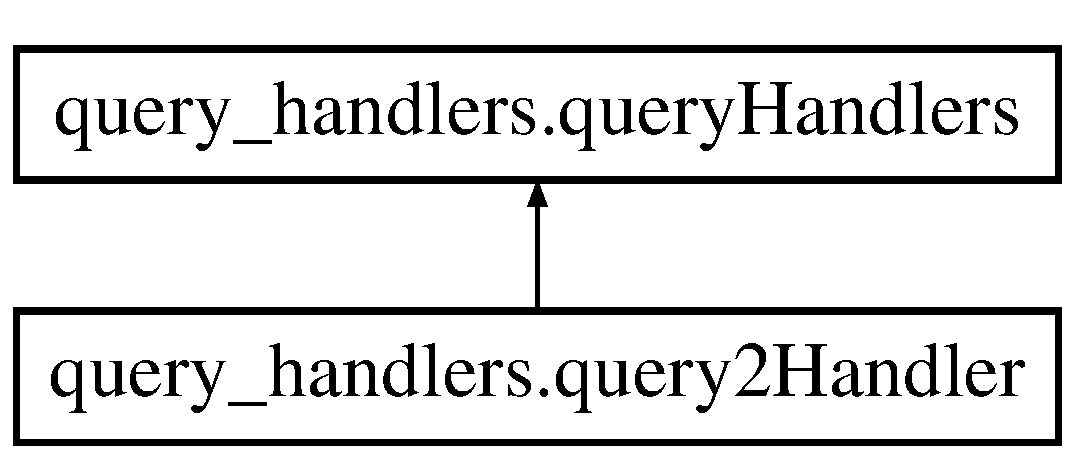
\includegraphics[height=2.000000cm]{classquery__handlers_1_1query2_handler}
\end{center}
\end{figure}
\subsection*{Public Member Functions}
\begin{DoxyCompactItemize}
\item 
\hyperlink{classquery__handlers_1_1query2_handler_a76beaa307feebaddfb1c0bc45432b3b8}{query2\+Handler} (int \+\_\+k)
\begin{DoxyCompactList}\small\item\em constructor \end{DoxyCompactList}\item 
void \hyperlink{classquery__handlers_1_1query2_handler_aea6272ec7e1d5c8806f95120c64f2d8c}{do\+Work} ()
\end{DoxyCompactItemize}


\subsection{Detailed Description}
Created by skwow on 10/27/2016. 

\subsection{Constructor \& Destructor Documentation}
\hypertarget{classquery__handlers_1_1query2_handler_a76beaa307feebaddfb1c0bc45432b3b8}{}\label{classquery__handlers_1_1query2_handler_a76beaa307feebaddfb1c0bc45432b3b8} 
\index{query\+\_\+handlers\+::query2\+Handler@{query\+\_\+handlers\+::query2\+Handler}!query2\+Handler@{query2\+Handler}}
\index{query2\+Handler@{query2\+Handler}!query\+\_\+handlers\+::query2\+Handler@{query\+\_\+handlers\+::query2\+Handler}}
\subsubsection{\texorpdfstring{query2\+Handler()}{query2Handler()}}
{\footnotesize\ttfamily query\+\_\+handlers.\+query2\+Handler.\+query2\+Handler (\begin{DoxyParamCaption}\item[{int}]{\+\_\+k }\end{DoxyParamCaption})}



constructor 



\subsection{Member Function Documentation}
\hypertarget{classquery__handlers_1_1query2_handler_aea6272ec7e1d5c8806f95120c64f2d8c}{}\label{classquery__handlers_1_1query2_handler_aea6272ec7e1d5c8806f95120c64f2d8c} 
\index{query\+\_\+handlers\+::query2\+Handler@{query\+\_\+handlers\+::query2\+Handler}!do\+Work@{do\+Work}}
\index{do\+Work@{do\+Work}!query\+\_\+handlers\+::query2\+Handler@{query\+\_\+handlers\+::query2\+Handler}}
\subsubsection{\texorpdfstring{do\+Work()}{doWork()}}
{\footnotesize\ttfamily void query\+\_\+handlers.\+query2\+Handler.\+do\+Work (\begin{DoxyParamCaption}{ }\end{DoxyParamCaption})}



The documentation for this class was generated from the following file\+:\begin{DoxyCompactItemize}
\item 
C\+:/\+Users/skwow/\+Documents/\+Git\+Hub/\+A\+P\+\_\+\+Project/src/query\+\_\+handlers/\hyperlink{query2_handler_8java}{query2\+Handler.\+java}\end{DoxyCompactItemize}

\hypertarget{classquery__handlers_1_1query3_handler}{}\section{query\+\_\+handlers.\+query3\+Handler Class Reference}
\label{classquery__handlers_1_1query3_handler}\index{query\+\_\+handlers.\+query3\+Handler@{query\+\_\+handlers.\+query3\+Handler}}
Inheritance diagram for query\+\_\+handlers.\+query3\+Handler\+:\begin{figure}[H]
\begin{center}
\leavevmode
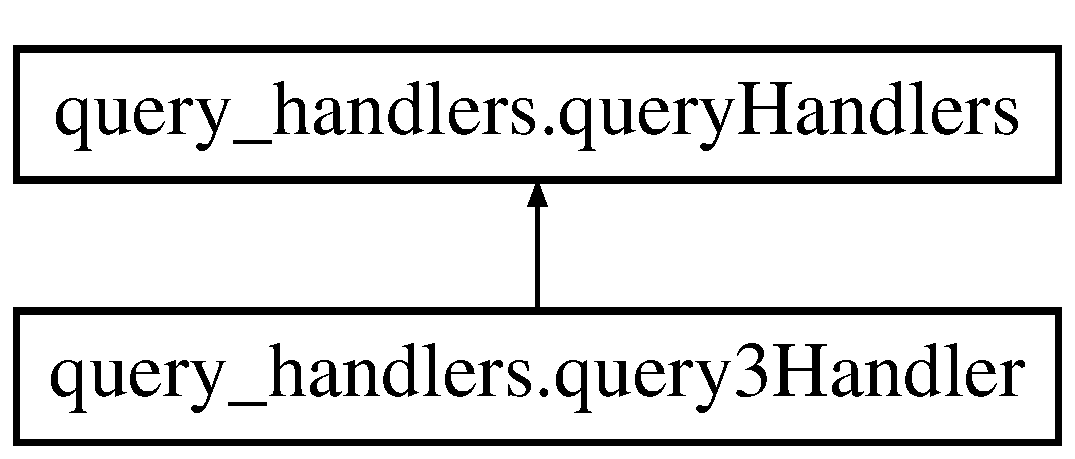
\includegraphics[height=2.000000cm]{classquery__handlers_1_1query3_handler}
\end{center}
\end{figure}
\subsection*{Public Member Functions}
\begin{DoxyCompactItemize}
\item 
\hyperlink{classquery__handlers_1_1query3_handler_aa874c1b45238e159383eb3d7ebf7efaa}{query3\+Handler} (String\mbox{[}$\,$\mbox{]} \+\_\+authors, int\mbox{[}$\,$\mbox{]} \+\_\+years)
\begin{DoxyCompactList}\small\item\em constructor \end{DoxyCompactList}\item 
void \hyperlink{classquery__handlers_1_1query3_handler_aca11896ec7db39b698a6c793837dc2fc}{do\+Work} ()
\begin{DoxyCompactList}\small\item\em use last 10\% of data to guess the number of publishables \end{DoxyCompactList}\item 
void \hyperlink{classquery__handlers_1_1query3_handler_a361412515dada11bc03c4f960a141d62}{sort} ()
\item 
void \hyperlink{classquery__handlers_1_1query3_handler_a19b8a0235fc333924fdc0948ea8cf856}{add} (\hyperlink{class_data_1_1publishables}{publishables} x)
\item 
void \hyperlink{classquery__handlers_1_1query3_handler_a62b09c05939d04c105e6f7f338931162}{print} ()
\item 
void \hyperlink{classquery__handlers_1_1query3_handler_a44fdc62828b748b374705c862515fe23}{show\+Result} ()
\begin{DoxyCompactList}\small\item\em sends result as 2d array to result\+Panel \end{DoxyCompactList}\end{DoxyCompactItemize}


\subsection{Detailed Description}
Created by skwow on 10/27/2016. saurabh kumar 2015088 prashant 2015072 

\subsection{Constructor \& Destructor Documentation}
\hypertarget{classquery__handlers_1_1query3_handler_aa874c1b45238e159383eb3d7ebf7efaa}{}\label{classquery__handlers_1_1query3_handler_aa874c1b45238e159383eb3d7ebf7efaa} 
\index{query\+\_\+handlers\+::query3\+Handler@{query\+\_\+handlers\+::query3\+Handler}!query3\+Handler@{query3\+Handler}}
\index{query3\+Handler@{query3\+Handler}!query\+\_\+handlers\+::query3\+Handler@{query\+\_\+handlers\+::query3\+Handler}}
\subsubsection{\texorpdfstring{query3\+Handler()}{query3Handler()}}
{\footnotesize\ttfamily query\+\_\+handlers.\+query3\+Handler.\+query3\+Handler (\begin{DoxyParamCaption}\item[{String \mbox{[}$\,$\mbox{]}}]{\+\_\+authors,  }\item[{int \mbox{[}$\,$\mbox{]}}]{\+\_\+years }\end{DoxyParamCaption})}



constructor 



\subsection{Member Function Documentation}
\hypertarget{classquery__handlers_1_1query3_handler_a19b8a0235fc333924fdc0948ea8cf856}{}\label{classquery__handlers_1_1query3_handler_a19b8a0235fc333924fdc0948ea8cf856} 
\index{query\+\_\+handlers\+::query3\+Handler@{query\+\_\+handlers\+::query3\+Handler}!add@{add}}
\index{add@{add}!query\+\_\+handlers\+::query3\+Handler@{query\+\_\+handlers\+::query3\+Handler}}
\subsubsection{\texorpdfstring{add()}{add()}}
{\footnotesize\ttfamily void query\+\_\+handlers.\+query3\+Handler.\+add (\begin{DoxyParamCaption}\item[{\hyperlink{class_data_1_1publishables}{publishables}}]{x }\end{DoxyParamCaption})}

\hypertarget{classquery__handlers_1_1query3_handler_aca11896ec7db39b698a6c793837dc2fc}{}\label{classquery__handlers_1_1query3_handler_aca11896ec7db39b698a6c793837dc2fc} 
\index{query\+\_\+handlers\+::query3\+Handler@{query\+\_\+handlers\+::query3\+Handler}!do\+Work@{do\+Work}}
\index{do\+Work@{do\+Work}!query\+\_\+handlers\+::query3\+Handler@{query\+\_\+handlers\+::query3\+Handler}}
\subsubsection{\texorpdfstring{do\+Work()}{doWork()}}
{\footnotesize\ttfamily void query\+\_\+handlers.\+query3\+Handler.\+do\+Work (\begin{DoxyParamCaption}{ }\end{DoxyParamCaption})}



use last 10\% of data to guess the number of publishables 

\hypertarget{classquery__handlers_1_1query3_handler_a62b09c05939d04c105e6f7f338931162}{}\label{classquery__handlers_1_1query3_handler_a62b09c05939d04c105e6f7f338931162} 
\index{query\+\_\+handlers\+::query3\+Handler@{query\+\_\+handlers\+::query3\+Handler}!print@{print}}
\index{print@{print}!query\+\_\+handlers\+::query3\+Handler@{query\+\_\+handlers\+::query3\+Handler}}
\subsubsection{\texorpdfstring{print()}{print()}}
{\footnotesize\ttfamily void query\+\_\+handlers.\+query3\+Handler.\+print (\begin{DoxyParamCaption}{ }\end{DoxyParamCaption})}

\hypertarget{classquery__handlers_1_1query3_handler_a44fdc62828b748b374705c862515fe23}{}\label{classquery__handlers_1_1query3_handler_a44fdc62828b748b374705c862515fe23} 
\index{query\+\_\+handlers\+::query3\+Handler@{query\+\_\+handlers\+::query3\+Handler}!show\+Result@{show\+Result}}
\index{show\+Result@{show\+Result}!query\+\_\+handlers\+::query3\+Handler@{query\+\_\+handlers\+::query3\+Handler}}
\subsubsection{\texorpdfstring{show\+Result()}{showResult()}}
{\footnotesize\ttfamily void query\+\_\+handlers.\+query3\+Handler.\+show\+Result (\begin{DoxyParamCaption}{ }\end{DoxyParamCaption})}



sends result as 2d array to result\+Panel 

\hypertarget{classquery__handlers_1_1query3_handler_a361412515dada11bc03c4f960a141d62}{}\label{classquery__handlers_1_1query3_handler_a361412515dada11bc03c4f960a141d62} 
\index{query\+\_\+handlers\+::query3\+Handler@{query\+\_\+handlers\+::query3\+Handler}!sort@{sort}}
\index{sort@{sort}!query\+\_\+handlers\+::query3\+Handler@{query\+\_\+handlers\+::query3\+Handler}}
\subsubsection{\texorpdfstring{sort()}{sort()}}
{\footnotesize\ttfamily void query\+\_\+handlers.\+query3\+Handler.\+sort (\begin{DoxyParamCaption}{ }\end{DoxyParamCaption})}



The documentation for this class was generated from the following file\+:\begin{DoxyCompactItemize}
\item 
C\+:/\+Users/skwow/\+Documents/\+Git\+Hub/\+A\+P\+\_\+\+Project/src/query\+\_\+handlers/\hyperlink{query3_handler_8java}{query3\+Handler.\+java}\end{DoxyCompactItemize}

\hypertarget{classquery__handlers_1_1query_handlers}{}\section{query\+\_\+handlers.\+query\+Handlers Class Reference}
\label{classquery__handlers_1_1query_handlers}\index{query\+\_\+handlers.\+query\+Handlers@{query\+\_\+handlers.\+query\+Handlers}}


template pattern. for all the 3 \hyperlink{classquery__handlers_1_1query_handlers}{query\+Handlers}  


Inheritance diagram for query\+\_\+handlers.\+query\+Handlers\+:\begin{figure}[H]
\begin{center}
\leavevmode
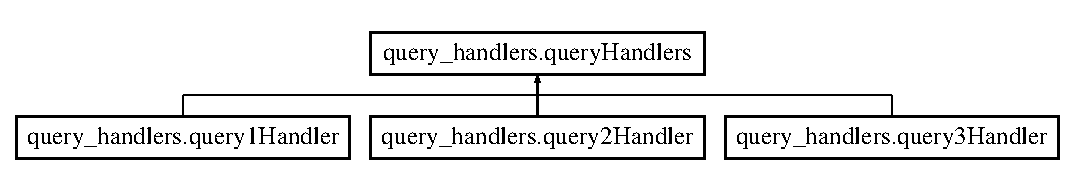
\includegraphics[height=1.904762cm]{classquery__handlers_1_1query_handlers}
\end{center}
\end{figure}
\subsection*{Public Member Functions}
\begin{DoxyCompactItemize}
\item 
final void \hyperlink{classquery__handlers_1_1query_handlers_a2ffd93ab8225b054b72f8a99b45bed2f}{perform} ()
\begin{DoxyCompactList}\small\item\em skeleton \end{DoxyCompactList}\end{DoxyCompactItemize}


\subsection{Detailed Description}
template pattern. for all the 3 \hyperlink{classquery__handlers_1_1query_handlers}{query\+Handlers} 

Created by skwow on 11/29/2016. saurabh kumar 2015088 prashant 2015072 

\subsection{Member Function Documentation}
\hypertarget{classquery__handlers_1_1query_handlers_a2ffd93ab8225b054b72f8a99b45bed2f}{}\label{classquery__handlers_1_1query_handlers_a2ffd93ab8225b054b72f8a99b45bed2f} 
\index{query\+\_\+handlers\+::query\+Handlers@{query\+\_\+handlers\+::query\+Handlers}!perform@{perform}}
\index{perform@{perform}!query\+\_\+handlers\+::query\+Handlers@{query\+\_\+handlers\+::query\+Handlers}}
\subsubsection{\texorpdfstring{perform()}{perform()}}
{\footnotesize\ttfamily final void query\+\_\+handlers.\+query\+Handlers.\+perform (\begin{DoxyParamCaption}{ }\end{DoxyParamCaption})}



skeleton 



The documentation for this class was generated from the following file\+:\begin{DoxyCompactItemize}
\item 
C\+:/\+Users/skwow/\+Documents/\+Git\+Hub/\+A\+P\+\_\+\+Project/src/query\+\_\+handlers/\hyperlink{query_handlers_8java}{query\+Handlers.\+java}\end{DoxyCompactItemize}

\hypertarget{class_g_u_i___elements_1_1query_panels}{}\section{G\+U\+I\+\_\+\+Elements.\+query\+Panels Class Reference}
\label{class_g_u_i___elements_1_1query_panels}\index{G\+U\+I\+\_\+\+Elements.\+query\+Panels@{G\+U\+I\+\_\+\+Elements.\+query\+Panels}}


template pattern. for all the different querypanels  


Inheritance diagram for G\+U\+I\+\_\+\+Elements.\+query\+Panels\+:\begin{figure}[H]
\begin{center}
\leavevmode
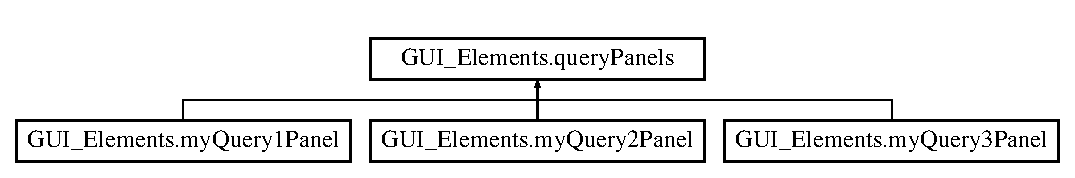
\includegraphics[height=1.944445cm]{class_g_u_i___elements_1_1query_panels}
\end{center}
\end{figure}
\subsection*{Public Member Functions}
\begin{DoxyCompactItemize}
\item 
final void \hyperlink{class_g_u_i___elements_1_1query_panels_accb5dae53ed500cf39ba1ce8833029fc}{prepare} ()
\begin{DoxyCompactList}\small\item\em skeleton \end{DoxyCompactList}\end{DoxyCompactItemize}


\subsection{Detailed Description}
template pattern. for all the different querypanels 

Created by skwow on 11/29/2016. saurabh kumar 2015088 prashant 2015072 

\subsection{Member Function Documentation}
\hypertarget{class_g_u_i___elements_1_1query_panels_accb5dae53ed500cf39ba1ce8833029fc}{}\label{class_g_u_i___elements_1_1query_panels_accb5dae53ed500cf39ba1ce8833029fc} 
\index{G\+U\+I\+\_\+\+Elements\+::query\+Panels@{G\+U\+I\+\_\+\+Elements\+::query\+Panels}!prepare@{prepare}}
\index{prepare@{prepare}!G\+U\+I\+\_\+\+Elements\+::query\+Panels@{G\+U\+I\+\_\+\+Elements\+::query\+Panels}}
\subsubsection{\texorpdfstring{prepare()}{prepare()}}
{\footnotesize\ttfamily final void G\+U\+I\+\_\+\+Elements.\+query\+Panels.\+prepare (\begin{DoxyParamCaption}{ }\end{DoxyParamCaption})}



skeleton 



The documentation for this class was generated from the following file\+:\begin{DoxyCompactItemize}
\item 
C\+:/\+Users/skwow/\+Documents/\+Git\+Hub/\+A\+P\+\_\+\+Project/src/\+G\+U\+I\+\_\+\+Elements/\hyperlink{query_panels_8java}{query\+Panels.\+java}\end{DoxyCompactItemize}

\hypertarget{class_g_u_i___elements_1_1result_panel}{}\section{G\+U\+I\+\_\+\+Elements.\+result\+Panel Class Reference}
\label{class_g_u_i___elements_1_1result_panel}\index{G\+U\+I\+\_\+\+Elements.\+result\+Panel@{G\+U\+I\+\_\+\+Elements.\+result\+Panel}}


contains output box for result  


\subsection*{Public Member Functions}
\begin{DoxyCompactItemize}
\item 
\hyperlink{class_g_u_i___elements_1_1result_panel_ae3658e3ae9e9685a8313ddc8f76426bf}{result\+Panel} ()
\item 
J\+Panel \hyperlink{class_g_u_i___elements_1_1result_panel_ad5c462dff38294c96ee565dc5f258566}{get\+Pane} ()
\item 
void \hyperlink{class_g_u_i___elements_1_1result_panel_abba17e8bbb434ee86c7f95d00167c99d}{prepare\+Buttons} ()
\end{DoxyCompactItemize}
\subsection*{Static Public Member Functions}
\begin{DoxyCompactItemize}
\item 
static void \hyperlink{class_g_u_i___elements_1_1result_panel_a1f5c577e0d7335cca042570a2d406c01}{update\+Data} (Object\mbox{[}$\,$\mbox{]}\mbox{[}$\,$\mbox{]} \+\_\+data, String\mbox{[}$\,$\mbox{]} col\+Data)
\item 
static void \hyperlink{class_g_u_i___elements_1_1result_panel_a9b7265b21d672434bb1d53273ea82590}{update\+Table} ()
\begin{DoxyCompactList}\small\item\em responsible for ensuring only 20 lines goes at a time \end{DoxyCompactList}\end{DoxyCompactItemize}


\subsection{Detailed Description}
contains output box for result 

Created by skwow on 10/27/2016. 

\subsection{Constructor \& Destructor Documentation}
\hypertarget{class_g_u_i___elements_1_1result_panel_ae3658e3ae9e9685a8313ddc8f76426bf}{}\label{class_g_u_i___elements_1_1result_panel_ae3658e3ae9e9685a8313ddc8f76426bf} 
\index{G\+U\+I\+\_\+\+Elements\+::result\+Panel@{G\+U\+I\+\_\+\+Elements\+::result\+Panel}!result\+Panel@{result\+Panel}}
\index{result\+Panel@{result\+Panel}!G\+U\+I\+\_\+\+Elements\+::result\+Panel@{G\+U\+I\+\_\+\+Elements\+::result\+Panel}}
\subsubsection{\texorpdfstring{result\+Panel()}{resultPanel()}}
{\footnotesize\ttfamily G\+U\+I\+\_\+\+Elements.\+result\+Panel.\+result\+Panel (\begin{DoxyParamCaption}{ }\end{DoxyParamCaption})}



\subsection{Member Function Documentation}
\hypertarget{class_g_u_i___elements_1_1result_panel_ad5c462dff38294c96ee565dc5f258566}{}\label{class_g_u_i___elements_1_1result_panel_ad5c462dff38294c96ee565dc5f258566} 
\index{G\+U\+I\+\_\+\+Elements\+::result\+Panel@{G\+U\+I\+\_\+\+Elements\+::result\+Panel}!get\+Pane@{get\+Pane}}
\index{get\+Pane@{get\+Pane}!G\+U\+I\+\_\+\+Elements\+::result\+Panel@{G\+U\+I\+\_\+\+Elements\+::result\+Panel}}
\subsubsection{\texorpdfstring{get\+Pane()}{getPane()}}
{\footnotesize\ttfamily J\+Panel G\+U\+I\+\_\+\+Elements.\+result\+Panel.\+get\+Pane (\begin{DoxyParamCaption}{ }\end{DoxyParamCaption})}

\hypertarget{class_g_u_i___elements_1_1result_panel_abba17e8bbb434ee86c7f95d00167c99d}{}\label{class_g_u_i___elements_1_1result_panel_abba17e8bbb434ee86c7f95d00167c99d} 
\index{G\+U\+I\+\_\+\+Elements\+::result\+Panel@{G\+U\+I\+\_\+\+Elements\+::result\+Panel}!prepare\+Buttons@{prepare\+Buttons}}
\index{prepare\+Buttons@{prepare\+Buttons}!G\+U\+I\+\_\+\+Elements\+::result\+Panel@{G\+U\+I\+\_\+\+Elements\+::result\+Panel}}
\subsubsection{\texorpdfstring{prepare\+Buttons()}{prepareButtons()}}
{\footnotesize\ttfamily void G\+U\+I\+\_\+\+Elements.\+result\+Panel.\+prepare\+Buttons (\begin{DoxyParamCaption}{ }\end{DoxyParamCaption})}

\hypertarget{class_g_u_i___elements_1_1result_panel_a1f5c577e0d7335cca042570a2d406c01}{}\label{class_g_u_i___elements_1_1result_panel_a1f5c577e0d7335cca042570a2d406c01} 
\index{G\+U\+I\+\_\+\+Elements\+::result\+Panel@{G\+U\+I\+\_\+\+Elements\+::result\+Panel}!update\+Data@{update\+Data}}
\index{update\+Data@{update\+Data}!G\+U\+I\+\_\+\+Elements\+::result\+Panel@{G\+U\+I\+\_\+\+Elements\+::result\+Panel}}
\subsubsection{\texorpdfstring{update\+Data()}{updateData()}}
{\footnotesize\ttfamily static void G\+U\+I\+\_\+\+Elements.\+result\+Panel.\+update\+Data (\begin{DoxyParamCaption}\item[{Object}]{\+\_\+data\mbox{[}$\,$\mbox{]}\mbox{[}$\,$\mbox{]},  }\item[{String \mbox{[}$\,$\mbox{]}}]{col\+Data }\end{DoxyParamCaption})\hspace{0.3cm}{\ttfamily [static]}}

\hypertarget{class_g_u_i___elements_1_1result_panel_a9b7265b21d672434bb1d53273ea82590}{}\label{class_g_u_i___elements_1_1result_panel_a9b7265b21d672434bb1d53273ea82590} 
\index{G\+U\+I\+\_\+\+Elements\+::result\+Panel@{G\+U\+I\+\_\+\+Elements\+::result\+Panel}!update\+Table@{update\+Table}}
\index{update\+Table@{update\+Table}!G\+U\+I\+\_\+\+Elements\+::result\+Panel@{G\+U\+I\+\_\+\+Elements\+::result\+Panel}}
\subsubsection{\texorpdfstring{update\+Table()}{updateTable()}}
{\footnotesize\ttfamily static void G\+U\+I\+\_\+\+Elements.\+result\+Panel.\+update\+Table (\begin{DoxyParamCaption}{ }\end{DoxyParamCaption})\hspace{0.3cm}{\ttfamily [static]}}



responsible for ensuring only 20 lines goes at a time 



The documentation for this class was generated from the following file\+:\begin{DoxyCompactItemize}
\item 
C\+:/\+Users/skwow/\+Documents/\+Git\+Hub/\+A\+P\+\_\+\+Project/src/\+G\+U\+I\+\_\+\+Elements/\hyperlink{result_panel_8java}{result\+Panel.\+java}\end{DoxyCompactItemize}

\chapter{File Documentation}
\hypertarget{data_8java}{}\section{C\+:/\+Users/skwow/\+Documents/\+Git\+Hub/\+A\+P\+\_\+\+Project/src/\+Data/data.java File Reference}
\label{data_8java}\index{C\+:/\+Users/skwow/\+Documents/\+Git\+Hub/\+A\+P\+\_\+\+Project/src/\+Data/data.\+java@{C\+:/\+Users/skwow/\+Documents/\+Git\+Hub/\+A\+P\+\_\+\+Project/src/\+Data/data.\+java}}
\subsection*{Classes}
\begin{DoxyCompactItemize}
\item 
class \hyperlink{class_data_1_1data}{Data.\+data}
\begin{DoxyCompactList}\small\item\em this class saves all the data parsed by parser \end{DoxyCompactList}\end{DoxyCompactItemize}
\subsection*{Packages}
\begin{DoxyCompactItemize}
\item 
package \hyperlink{namespace_data}{Data}
\end{DoxyCompactItemize}

\hypertarget{publishables_8java}{}\section{C\+:/\+Users/skwow/\+Documents/\+Git\+Hub/\+A\+P\+\_\+\+Project/src/\+Data/publishables.java File Reference}
\label{publishables_8java}\index{C\+:/\+Users/skwow/\+Documents/\+Git\+Hub/\+A\+P\+\_\+\+Project/src/\+Data/publishables.\+java@{C\+:/\+Users/skwow/\+Documents/\+Git\+Hub/\+A\+P\+\_\+\+Project/src/\+Data/publishables.\+java}}
\subsection*{Classes}
\begin{DoxyCompactItemize}
\item 
class \hyperlink{class_data_1_1publishables}{Data.\+publishables}
\begin{DoxyCompactList}\small\item\em publishale comprises of all thethigs in the xml \end{DoxyCompactList}\end{DoxyCompactItemize}
\subsection*{Packages}
\begin{DoxyCompactItemize}
\item 
package \hyperlink{namespace_data}{Data}
\end{DoxyCompactItemize}

\hypertarget{loading_screen_8java}{}\section{C\+:/\+Users/skwow/\+Documents/\+Git\+Hub/\+A\+P\+\_\+\+Project/src/\+G\+U\+I\+\_\+\+Elements/loading\+Screen.java File Reference}
\label{loading_screen_8java}\index{C\+:/\+Users/skwow/\+Documents/\+Git\+Hub/\+A\+P\+\_\+\+Project/src/\+G\+U\+I\+\_\+\+Elements/loading\+Screen.\+java@{C\+:/\+Users/skwow/\+Documents/\+Git\+Hub/\+A\+P\+\_\+\+Project/src/\+G\+U\+I\+\_\+\+Elements/loading\+Screen.\+java}}
\subsection*{Classes}
\begin{DoxyCompactItemize}
\item 
class \hyperlink{class_g_u_i___elements_1_1loading_screen}{G\+U\+I\+\_\+\+Elements.\+loading\+Screen}
\begin{DoxyCompactList}\small\item\em loading screen that pops up while reading xml file. \end{DoxyCompactList}\end{DoxyCompactItemize}
\subsection*{Packages}
\begin{DoxyCompactItemize}
\item 
package \hyperlink{namespace_g_u_i___elements}{G\+U\+I\+\_\+\+Elements}
\end{DoxyCompactItemize}

\hypertarget{my_frame_8java}{}\section{C\+:/\+Users/skwow/\+Documents/\+Git\+Hub/\+A\+P\+\_\+\+Project/src/\+G\+U\+I\+\_\+\+Elements/my\+Frame.java File Reference}
\label{my_frame_8java}\index{C\+:/\+Users/skwow/\+Documents/\+Git\+Hub/\+A\+P\+\_\+\+Project/src/\+G\+U\+I\+\_\+\+Elements/my\+Frame.\+java@{C\+:/\+Users/skwow/\+Documents/\+Git\+Hub/\+A\+P\+\_\+\+Project/src/\+G\+U\+I\+\_\+\+Elements/my\+Frame.\+java}}
\subsection*{Classes}
\begin{DoxyCompactItemize}
\item 
class \hyperlink{class_g_u_i___elements_1_1my_frame}{G\+U\+I\+\_\+\+Elements.\+my\+Frame}
\begin{DoxyCompactList}\small\item\em main G\+UI frame \end{DoxyCompactList}\end{DoxyCompactItemize}
\subsection*{Packages}
\begin{DoxyCompactItemize}
\item 
package \hyperlink{namespace_g_u_i___elements}{G\+U\+I\+\_\+\+Elements}
\end{DoxyCompactItemize}

\hypertarget{my_panel_8java}{}\section{C\+:/\+Users/skwow/\+Documents/\+Git\+Hub/\+A\+P\+\_\+\+Project/src/\+G\+U\+I\+\_\+\+Elements/my\+Panel.java File Reference}
\label{my_panel_8java}\index{C\+:/\+Users/skwow/\+Documents/\+Git\+Hub/\+A\+P\+\_\+\+Project/src/\+G\+U\+I\+\_\+\+Elements/my\+Panel.\+java@{C\+:/\+Users/skwow/\+Documents/\+Git\+Hub/\+A\+P\+\_\+\+Project/src/\+G\+U\+I\+\_\+\+Elements/my\+Panel.\+java}}
\subsection*{Classes}
\begin{DoxyCompactItemize}
\item 
class \hyperlink{class_g_u_i___elements_1_1my_panel}{G\+U\+I\+\_\+\+Elements.\+my\+Panel}
\begin{DoxyCompactList}\small\item\em main panel inside \hyperlink{class_g_u_i___elements_1_1my_frame}{my\+Frame} \end{DoxyCompactList}\end{DoxyCompactItemize}
\subsection*{Packages}
\begin{DoxyCompactItemize}
\item 
package \hyperlink{namespace_g_u_i___elements}{G\+U\+I\+\_\+\+Elements}
\end{DoxyCompactItemize}

\hypertarget{my_query1_panel_8java}{}\section{C\+:/\+Users/skwow/\+Documents/\+Git\+Hub/\+A\+P\+\_\+\+Project/src/\+G\+U\+I\+\_\+\+Elements/my\+Query1\+Panel.java File Reference}
\label{my_query1_panel_8java}\index{C\+:/\+Users/skwow/\+Documents/\+Git\+Hub/\+A\+P\+\_\+\+Project/src/\+G\+U\+I\+\_\+\+Elements/my\+Query1\+Panel.\+java@{C\+:/\+Users/skwow/\+Documents/\+Git\+Hub/\+A\+P\+\_\+\+Project/src/\+G\+U\+I\+\_\+\+Elements/my\+Query1\+Panel.\+java}}
\subsection*{Classes}
\begin{DoxyCompactItemize}
\item 
class \hyperlink{class_g_u_i___elements_1_1my_query1_panel}{G\+U\+I\+\_\+\+Elements.\+my\+Query1\+Panel}
\end{DoxyCompactItemize}
\subsection*{Packages}
\begin{DoxyCompactItemize}
\item 
package \hyperlink{namespace_g_u_i___elements}{G\+U\+I\+\_\+\+Elements}
\end{DoxyCompactItemize}

\hypertarget{my_query2_panel_8java}{}\section{C\+:/\+Users/skwow/\+Documents/\+Git\+Hub/\+A\+P\+\_\+\+Project/src/\+G\+U\+I\+\_\+\+Elements/my\+Query2\+Panel.java File Reference}
\label{my_query2_panel_8java}\index{C\+:/\+Users/skwow/\+Documents/\+Git\+Hub/\+A\+P\+\_\+\+Project/src/\+G\+U\+I\+\_\+\+Elements/my\+Query2\+Panel.\+java@{C\+:/\+Users/skwow/\+Documents/\+Git\+Hub/\+A\+P\+\_\+\+Project/src/\+G\+U\+I\+\_\+\+Elements/my\+Query2\+Panel.\+java}}
\subsection*{Classes}
\begin{DoxyCompactItemize}
\item 
class \hyperlink{class_g_u_i___elements_1_1my_query2_panel}{G\+U\+I\+\_\+\+Elements.\+my\+Query2\+Panel}
\end{DoxyCompactItemize}
\subsection*{Packages}
\begin{DoxyCompactItemize}
\item 
package \hyperlink{namespace_g_u_i___elements}{G\+U\+I\+\_\+\+Elements}
\end{DoxyCompactItemize}

\hypertarget{my_query3_panel_8java}{}\section{C\+:/\+Users/skwow/\+Documents/\+Git\+Hub/\+A\+P\+\_\+\+Project/src/\+G\+U\+I\+\_\+\+Elements/my\+Query3\+Panel.java File Reference}
\label{my_query3_panel_8java}\index{C\+:/\+Users/skwow/\+Documents/\+Git\+Hub/\+A\+P\+\_\+\+Project/src/\+G\+U\+I\+\_\+\+Elements/my\+Query3\+Panel.\+java@{C\+:/\+Users/skwow/\+Documents/\+Git\+Hub/\+A\+P\+\_\+\+Project/src/\+G\+U\+I\+\_\+\+Elements/my\+Query3\+Panel.\+java}}
\subsection*{Classes}
\begin{DoxyCompactItemize}
\item 
class \hyperlink{class_g_u_i___elements_1_1my_query3_panel}{G\+U\+I\+\_\+\+Elements.\+my\+Query3\+Panel}
\end{DoxyCompactItemize}
\subsection*{Packages}
\begin{DoxyCompactItemize}
\item 
package \hyperlink{namespace_g_u_i___elements}{G\+U\+I\+\_\+\+Elements}
\end{DoxyCompactItemize}

\hypertarget{query_panels_8java}{}\section{C\+:/\+Users/skwow/\+Documents/\+Git\+Hub/\+A\+P\+\_\+\+Project/src/\+G\+U\+I\+\_\+\+Elements/query\+Panels.java File Reference}
\label{query_panels_8java}\index{C\+:/\+Users/skwow/\+Documents/\+Git\+Hub/\+A\+P\+\_\+\+Project/src/\+G\+U\+I\+\_\+\+Elements/query\+Panels.\+java@{C\+:/\+Users/skwow/\+Documents/\+Git\+Hub/\+A\+P\+\_\+\+Project/src/\+G\+U\+I\+\_\+\+Elements/query\+Panels.\+java}}
\subsection*{Classes}
\begin{DoxyCompactItemize}
\item 
class \hyperlink{class_g_u_i___elements_1_1query_panels}{G\+U\+I\+\_\+\+Elements.\+query\+Panels}
\begin{DoxyCompactList}\small\item\em template pattern. for all the different querypanels \end{DoxyCompactList}\end{DoxyCompactItemize}
\subsection*{Packages}
\begin{DoxyCompactItemize}
\item 
package \hyperlink{namespace_g_u_i___elements}{G\+U\+I\+\_\+\+Elements}
\end{DoxyCompactItemize}

\hypertarget{result_panel_8java}{}\section{C\+:/\+Users/skwow/\+Documents/\+Git\+Hub/\+A\+P\+\_\+\+Project/src/\+G\+U\+I\+\_\+\+Elements/result\+Panel.java File Reference}
\label{result_panel_8java}\index{C\+:/\+Users/skwow/\+Documents/\+Git\+Hub/\+A\+P\+\_\+\+Project/src/\+G\+U\+I\+\_\+\+Elements/result\+Panel.\+java@{C\+:/\+Users/skwow/\+Documents/\+Git\+Hub/\+A\+P\+\_\+\+Project/src/\+G\+U\+I\+\_\+\+Elements/result\+Panel.\+java}}
\subsection*{Classes}
\begin{DoxyCompactItemize}
\item 
class \hyperlink{class_g_u_i___elements_1_1result_panel}{G\+U\+I\+\_\+\+Elements.\+result\+Panel}
\begin{DoxyCompactList}\small\item\em contains output box for result \end{DoxyCompactList}\end{DoxyCompactItemize}
\subsection*{Packages}
\begin{DoxyCompactItemize}
\item 
package \hyperlink{namespace_g_u_i___elements}{G\+U\+I\+\_\+\+Elements}
\end{DoxyCompactItemize}

\hypertarget{main_class_8java}{}\section{C\+:/\+Users/skwow/\+Documents/\+Git\+Hub/\+A\+P\+\_\+\+Project/src/main\+\_\+\+Class/main\+Class.java File Reference}
\label{main_class_8java}\index{C\+:/\+Users/skwow/\+Documents/\+Git\+Hub/\+A\+P\+\_\+\+Project/src/main\+\_\+\+Class/main\+Class.\+java@{C\+:/\+Users/skwow/\+Documents/\+Git\+Hub/\+A\+P\+\_\+\+Project/src/main\+\_\+\+Class/main\+Class.\+java}}
\subsection*{Classes}
\begin{DoxyCompactItemize}
\item 
class \hyperlink{classmain___class_1_1main_class}{main\+\_\+\+Class.\+main\+Class}
\begin{DoxyCompactList}\small\item\em this is simply the main class \end{DoxyCompactList}\end{DoxyCompactItemize}
\subsection*{Packages}
\begin{DoxyCompactItemize}
\item 
package \hyperlink{namespacemain___class}{main\+\_\+\+Class}
\end{DoxyCompactItemize}

\hypertarget{query1_handler_8java}{}\section{C\+:/\+Users/skwow/\+Documents/\+Git\+Hub/\+A\+P\+\_\+\+Project/src/query\+\_\+handlers/query1\+Handler.java File Reference}
\label{query1_handler_8java}\index{C\+:/\+Users/skwow/\+Documents/\+Git\+Hub/\+A\+P\+\_\+\+Project/src/query\+\_\+handlers/query1\+Handler.\+java@{C\+:/\+Users/skwow/\+Documents/\+Git\+Hub/\+A\+P\+\_\+\+Project/src/query\+\_\+handlers/query1\+Handler.\+java}}
\subsection*{Classes}
\begin{DoxyCompactItemize}
\item 
class \hyperlink{classquery__handlers_1_1query1_handler}{query\+\_\+handlers.\+query1\+Handler}
\end{DoxyCompactItemize}
\subsection*{Packages}
\begin{DoxyCompactItemize}
\item 
package \hyperlink{namespacequery__handlers}{query\+\_\+handlers}
\end{DoxyCompactItemize}

\hypertarget{query2_handler_8java}{}\section{C\+:/\+Users/skwow/\+Documents/\+Git\+Hub/\+A\+P\+\_\+\+Project/src/query\+\_\+handlers/query2\+Handler.java File Reference}
\label{query2_handler_8java}\index{C\+:/\+Users/skwow/\+Documents/\+Git\+Hub/\+A\+P\+\_\+\+Project/src/query\+\_\+handlers/query2\+Handler.\+java@{C\+:/\+Users/skwow/\+Documents/\+Git\+Hub/\+A\+P\+\_\+\+Project/src/query\+\_\+handlers/query2\+Handler.\+java}}
\subsection*{Classes}
\begin{DoxyCompactItemize}
\item 
class \hyperlink{classquery__handlers_1_1query2_handler}{query\+\_\+handlers.\+query2\+Handler}
\end{DoxyCompactItemize}
\subsection*{Packages}
\begin{DoxyCompactItemize}
\item 
package \hyperlink{namespacequery__handlers}{query\+\_\+handlers}
\end{DoxyCompactItemize}

\hypertarget{query3_handler_8java}{}\section{C\+:/\+Users/skwow/\+Documents/\+Git\+Hub/\+A\+P\+\_\+\+Project/src/query\+\_\+handlers/query3\+Handler.java File Reference}
\label{query3_handler_8java}\index{C\+:/\+Users/skwow/\+Documents/\+Git\+Hub/\+A\+P\+\_\+\+Project/src/query\+\_\+handlers/query3\+Handler.\+java@{C\+:/\+Users/skwow/\+Documents/\+Git\+Hub/\+A\+P\+\_\+\+Project/src/query\+\_\+handlers/query3\+Handler.\+java}}
\subsection*{Classes}
\begin{DoxyCompactItemize}
\item 
class \hyperlink{classquery__handlers_1_1query3_handler}{query\+\_\+handlers.\+query3\+Handler}
\end{DoxyCompactItemize}
\subsection*{Packages}
\begin{DoxyCompactItemize}
\item 
package \hyperlink{namespacequery__handlers}{query\+\_\+handlers}
\end{DoxyCompactItemize}

\hypertarget{query_handlers_8java}{}\section{C\+:/\+Users/skwow/\+Documents/\+Git\+Hub/\+A\+P\+\_\+\+Project/src/query\+\_\+handlers/query\+Handlers.java File Reference}
\label{query_handlers_8java}\index{C\+:/\+Users/skwow/\+Documents/\+Git\+Hub/\+A\+P\+\_\+\+Project/src/query\+\_\+handlers/query\+Handlers.\+java@{C\+:/\+Users/skwow/\+Documents/\+Git\+Hub/\+A\+P\+\_\+\+Project/src/query\+\_\+handlers/query\+Handlers.\+java}}
\subsection*{Classes}
\begin{DoxyCompactItemize}
\item 
class \hyperlink{classquery__handlers_1_1query_handlers}{query\+\_\+handlers.\+query\+Handlers}
\begin{DoxyCompactList}\small\item\em template pattern. for all the 3 \hyperlink{classquery__handlers_1_1query_handlers}{query\+Handlers} \end{DoxyCompactList}\end{DoxyCompactItemize}
\subsection*{Packages}
\begin{DoxyCompactItemize}
\item 
package \hyperlink{namespacequery__handlers}{query\+\_\+handlers}
\end{DoxyCompactItemize}

\hypertarget{entity_resolver_8java}{}\section{C\+:/\+Users/skwow/\+Documents/\+Git\+Hub/\+A\+P\+\_\+\+Project/src/utilities/entity\+Resolver.java File Reference}
\label{entity_resolver_8java}\index{C\+:/\+Users/skwow/\+Documents/\+Git\+Hub/\+A\+P\+\_\+\+Project/src/utilities/entity\+Resolver.\+java@{C\+:/\+Users/skwow/\+Documents/\+Git\+Hub/\+A\+P\+\_\+\+Project/src/utilities/entity\+Resolver.\+java}}
\subsection*{Classes}
\begin{DoxyCompactItemize}
\item 
class \hyperlink{classutilities_1_1entity_resolver}{utilities.\+entity\+Resolver}
\begin{DoxyCompactList}\small\item\em a tool class for entity resolution \end{DoxyCompactList}\end{DoxyCompactItemize}
\subsection*{Packages}
\begin{DoxyCompactItemize}
\item 
package \hyperlink{namespaceutilities}{utilities}
\end{DoxyCompactItemize}

\hypertarget{my_own_exeption_8java}{}\section{C\+:/\+Users/skwow/\+Documents/\+Git\+Hub/\+A\+P\+\_\+\+Project/src/utilities/my\+Own\+Exeption.java File Reference}
\label{my_own_exeption_8java}\index{C\+:/\+Users/skwow/\+Documents/\+Git\+Hub/\+A\+P\+\_\+\+Project/src/utilities/my\+Own\+Exeption.\+java@{C\+:/\+Users/skwow/\+Documents/\+Git\+Hub/\+A\+P\+\_\+\+Project/src/utilities/my\+Own\+Exeption.\+java}}
\subsection*{Classes}
\begin{DoxyCompactItemize}
\item 
class \hyperlink{classutilities_1_1my_own_exeption}{utilities.\+my\+Own\+Exeption}
\begin{DoxyCompactList}\small\item\em this is meant for exception handling by creating dialog box. \end{DoxyCompactList}\end{DoxyCompactItemize}
\subsection*{Packages}
\begin{DoxyCompactItemize}
\item 
package \hyperlink{namespaceutilities}{utilities}
\end{DoxyCompactItemize}

\hypertarget{parser_8java}{}\section{C\+:/\+Users/skwow/\+Documents/\+Git\+Hub/\+A\+P\+\_\+\+Project/src/utilities/parser.java File Reference}
\label{parser_8java}\index{C\+:/\+Users/skwow/\+Documents/\+Git\+Hub/\+A\+P\+\_\+\+Project/src/utilities/parser.\+java@{C\+:/\+Users/skwow/\+Documents/\+Git\+Hub/\+A\+P\+\_\+\+Project/src/utilities/parser.\+java}}
\subsection*{Classes}
\begin{DoxyCompactItemize}
\item 
class \hyperlink{classutilities_1_1parser}{utilities.\+parser}
\begin{DoxyCompactList}\small\item\em this class parses the xml class \end{DoxyCompactList}\end{DoxyCompactItemize}
\subsection*{Packages}
\begin{DoxyCompactItemize}
\item 
package \hyperlink{namespaceutilities}{utilities}
\end{DoxyCompactItemize}

%--- End generated contents ---

% Index
\backmatter
\newpage
\phantomsection
\clearemptydoublepage
\addcontentsline{toc}{chapter}{Index}
\printindex

\end{document}
